%%%%%%%%%%%%%%%%%%%%%%%%%%%%%%%%%%%%%%%%%%%%%%%
%%% DISCLAIMER: The original template for this
%%% file can be found at:
%%%
%%% https://www.overleaf.com/latex/templates/report-template-stima-laborations-overleaf-v1-dot-0/jtctxkqjnjdz
%%%
%%% Template for lab reports for CS341 @ IITB
%%%%%%%%%%%%%%%%%%%%%%%%%%%%%%%%%%%%%%%%%%%%%%%

%%%%%%%%%%%%%%%%%%%%%%%%%%%%%% Sets the document class for the document
% Openany is added to remove the book style of starting every new chapter on an odd page (not needed for reports)
\documentclass[11pt, swedish, openany]{book}

%%%%%%%%%%%%%%%%%%%%%%%%%%%%%% Loading packages that alter the style
\usepackage[]{graphicx}
\usepackage[]{color}
\usepackage{alltt}
\usepackage[T1]{fontenc}
\usepackage[utf8]{inputenc}
\usepackage{float}
\usepackage{multirow}
\usepackage{tablefootnote}
\usepackage{wrapfig}
\usepackage{amsmath}
\usepackage{placeins}

\setcounter{secnumdepth}{3}
\setcounter{tocdepth}{3}
\setlength{\parskip}{\smallskipamount}
\setlength{\parindent}{0pt}

% Set page margins
\usepackage[top=100pt, bottom=100pt, left=60pt, right=60pt]{geometry}

% Package used for placeholder text
\usepackage{lipsum}

% Prevents LaTeX from filling out a page to the bottom
\raggedbottom

% Adding both languages, Swedish and English, so they can be used intermittently in for example abstracts.
\usepackage[swedish, english]{babel}

% All page numbers positioned at the bottom of the page
\usepackage{fancyhdr}
\fancyhf{} % clear all header and footers
\fancyfoot[C]{\thepage}
\renewcommand{\headrulewidth}{0pt} % remove the header rule
\pagestyle{fancy}

% Changes the style of chapter headings
\usepackage{titlesec}
\titleformat{\chapter}{\normalfont\LARGE\bfseries}{Part \thechapter:}{0.5em}{}
% Change distance between chapter header and text
\titlespacing{\chapter}{0pt}{50pt}{2\baselineskip}

% Adds table captions above the table per default
\usepackage{float}
\floatstyle{plaintop}
\restylefloat{table}

% Adds space between caption and table
\usepackage[tableposition=top]{caption}

% Adds hyperlinks to references and ToC
\usepackage{hyperref}
\hypersetup{hidelinks, linkcolor = blue} % Changes the link color to black and hides the hideous red border that usually is created

% If multiple images are to be added, a folder (path) with all the images can be added here
\graphicspath{{images/}}

% Separates the first part of the report/thesis in Roman numerals
\frontmatter


%%%%%%%%%%%%%%%%%%%%%%%%%%%%%% Starts the document
\begin{document}

%%% Selects the language to be used for the first couple of pages
\selectlanguage{english}

%%%%% Adds the title page
\begin{titlepage}
    \clearpage\thispagestyle{empty}
    \centering
    \vspace{2cm}

    % Titles
    {\large CS341: Computer Architecture Lab \par}
    \vspace{4cm}
    {\Huge \textbf{Lab Assignment 4} \par}
    \vspace{0.2cm}
    {\huge \textbf{Report} \par}
    \vspace{1.2cm}
    {\normalsize Devansh Jain \texttt{(190100044)} \par}
    \vfill
    {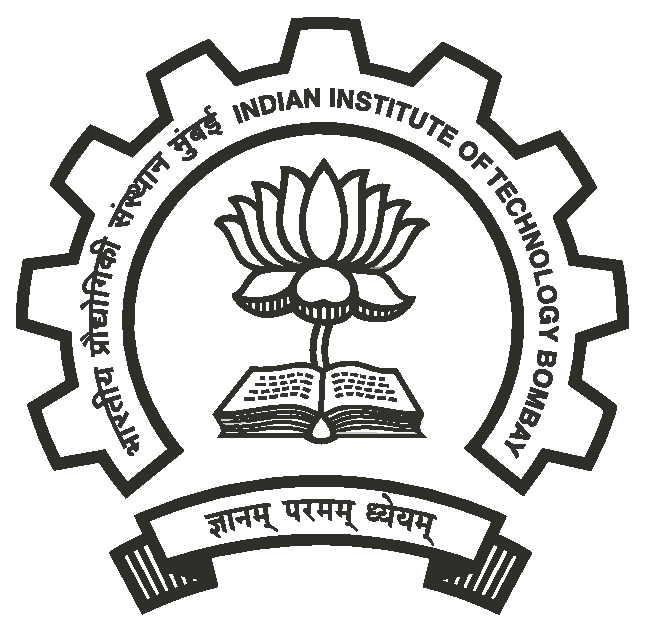
\includegraphics[scale=0.30]{iitb_logo/iitb_logo.eps} \par}
    \vspace{0.5cm}
    {\normalsize
        Department of Computer Science and Engineering \\
        Indian Institute of Technology Bombay \par}
    {\normalsize 2021-2022 \par}

\end{titlepage}

% Adds a table of contents
\tableofcontents{}

\clearpage

% Uncomment the following three rows for a table of figures and/or tables as they are not needed for lab reports
% \listoffigures
% \clearpage
% \listoftables

\mainmatter
\setcounter{chapter}{-1}

%%%%%%%%%%%%%%%%%%%%%%%%%%%%%%%%%%%%%%%%%%%%%%%%
%% Abstract
%%%%%%%%%%%%%%%%%%%%%%%%%%%%%%%%%%%%%%%%%%%%%%%%
\chapter*{\centerline{Abstract}}
Summarize the objective of the lab, what experiments you have conducted, what were the results that you have obtained in a clear and concise manner. Numbers matter, not just words only, for ex. \emph{very high}, \emph{slow} etc.

%%%%%%%%%%%%%%%%%%%%%%%%%%%%%%%%%%%%%%%%%%%%%%%%
%% Part 0: Getting Things Ready
%%%%%%%%%%%%%%%%%%%%%%%%%%%%%%%%%%%%%%%%%%%%%%%%
\chapter{Getting Things Ready}
\section*{Install \texttt{Intel VTune Profiler}}
Installed successfully using the stand-alone app using offline installer script present in this \hyperlink{https://software.intel.com/content/www/us/en/develop/tools/oneapi/components/vtune-profiler/download.html?operatingsystem=linux&distributions=webdownload&options=offline}{link}.

It was pretty easy to install \texttt{VTune} using the script. \\
While installing it showed that I didn't have \texttt{XCB} and \texttt{DRM} packages installed. Upon checking, I confirmed that they were already present. \\
Even though it failed prerequisites, there was a next option. I didn't face any issues for the rest of installation process. \\
From start to end, it took around 10-12 minutes to have the application installed, followed by 3-5 minutes for tutorial.

\section*{Install \texttt{Docker}}
Had docker setup from other projects. \\
Version: 20.10.9

\section*{Pull \texttt{ChampSim} Image}
Pulled \texttt{0xd3ba/champsim-lab:latest}

%%%%%%%%%%%%%%%%%%%%%%%%%%%%%%%%%%%%%%%%%%%%%%%%
%% Part 1: Profiling with VTune
%%%%%%%%%%%%%%%%%%%%%%%%%%%%%%%%%%%%%%%%%%%%%%%%
\chapter{Profiling with VTune}
\section{\texttt{bfs.cpp}}

\subsection*{Performance Snapshot}
\begin{itemize}
    \item IPC: 1.830
    \item Logical Core Utilization: 8.2\% (0.979 out of 12)
    \item Physical Core Utilization: 16.2\% (0.973 of 6)
    \item Memory bound: 32.0\% of Pipeline slots
\end{itemize}

\begin{figure}[H]
    \centering
    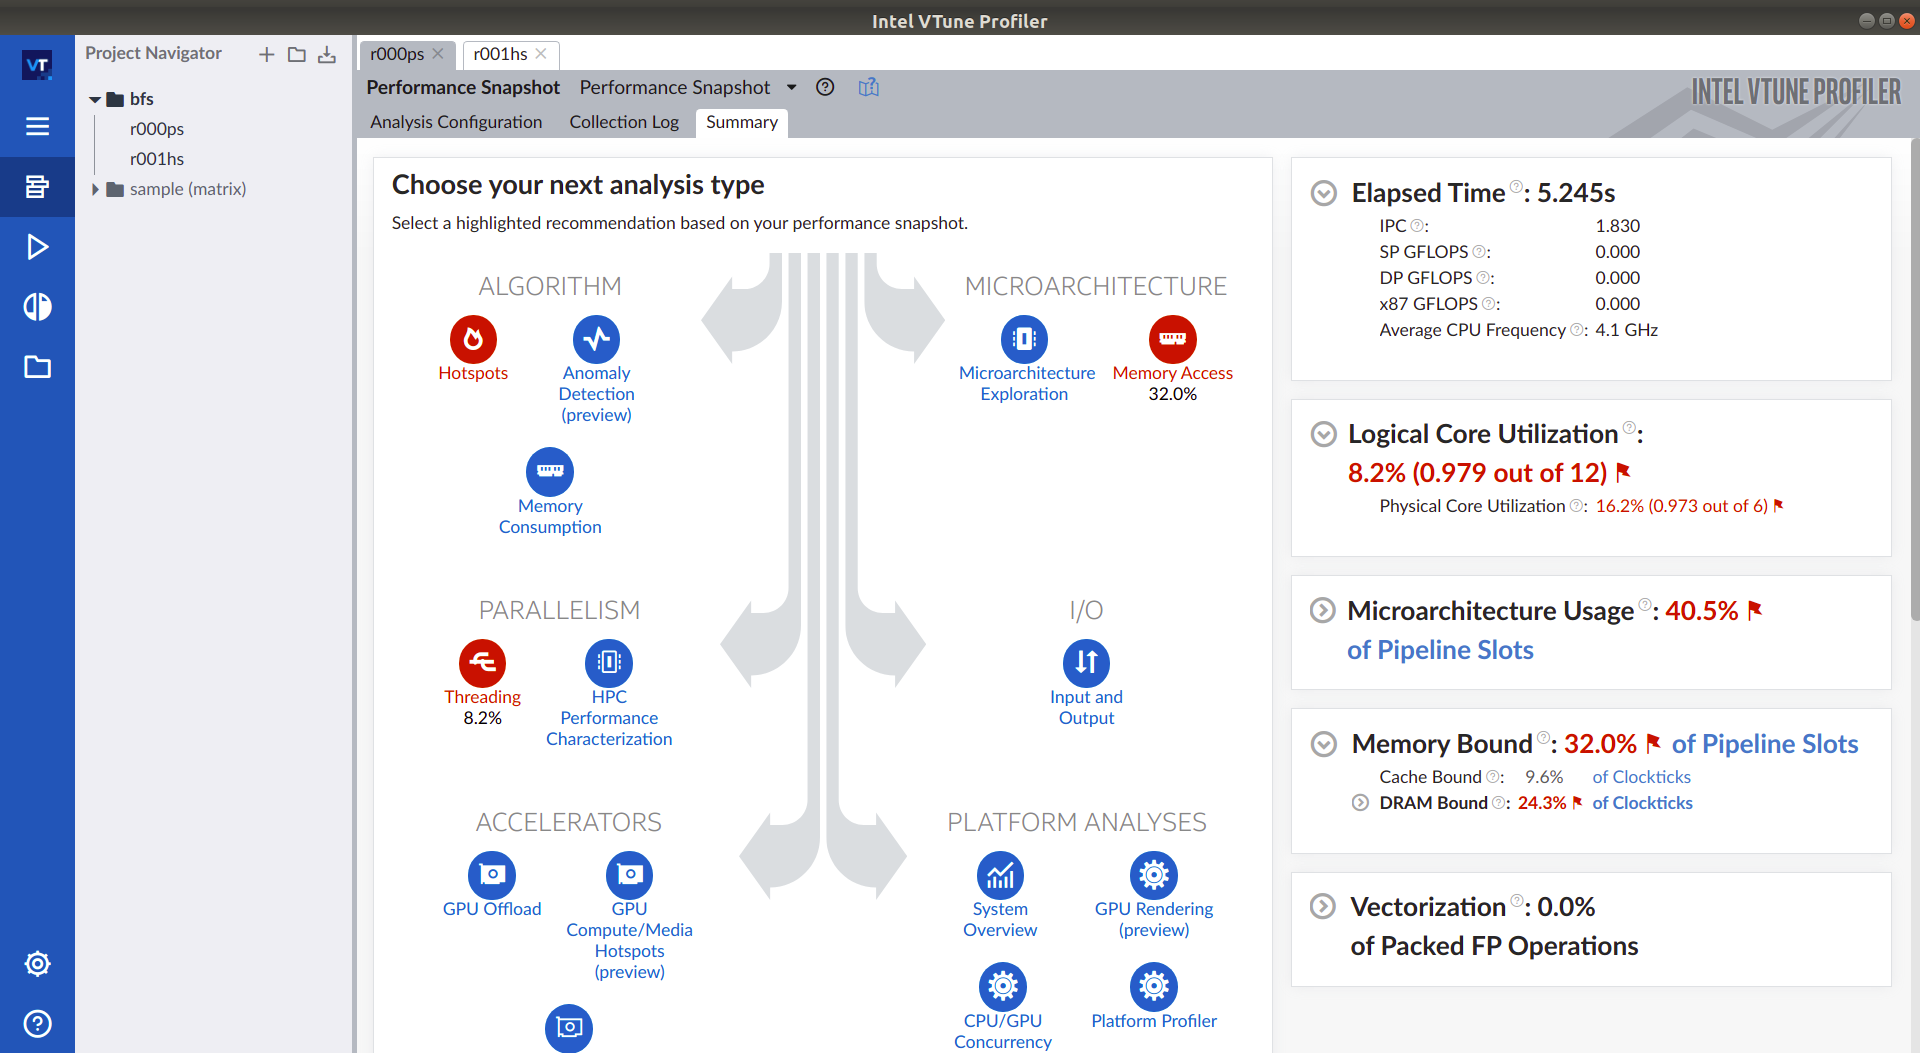
\includegraphics[scale=0.25]{vtune/bfs/ps.png}
    \caption{Performance Snapshot for \texttt{bfs.cpp}}
\end{figure}

\newpage
\subsection*{Top 5 Functions by CPU Time}
\begin{table}[H]
    \begin{tabular}{||l|l||c||}
        \hline
        Function                                                                      & Module                & CPU Time \\
        \hline
        \texttt{bfs}                                                                  & \texttt{bfs.o}        & 2.621s   \\
        \texttt{main}                                                                 & \texttt{bfs.o}        & 1.156s   \\
        \texttt{\_int\_free}                                                          & \texttt{libc-2.27.so} & 0.236s   \\
        \texttt{\_int\_malloc}                                                        & \texttt{libc-2.27.so} & 0.154s   \\
        \texttt{\_\_gnu\_cxx::new\_allocator<Node*>::construct<Node*, Node* const\&>} & \texttt{bfs.o}        & 0.124s   \\
        \hline
    \end{tabular}
\end{table}

\begin{figure}[H]
    \centering
    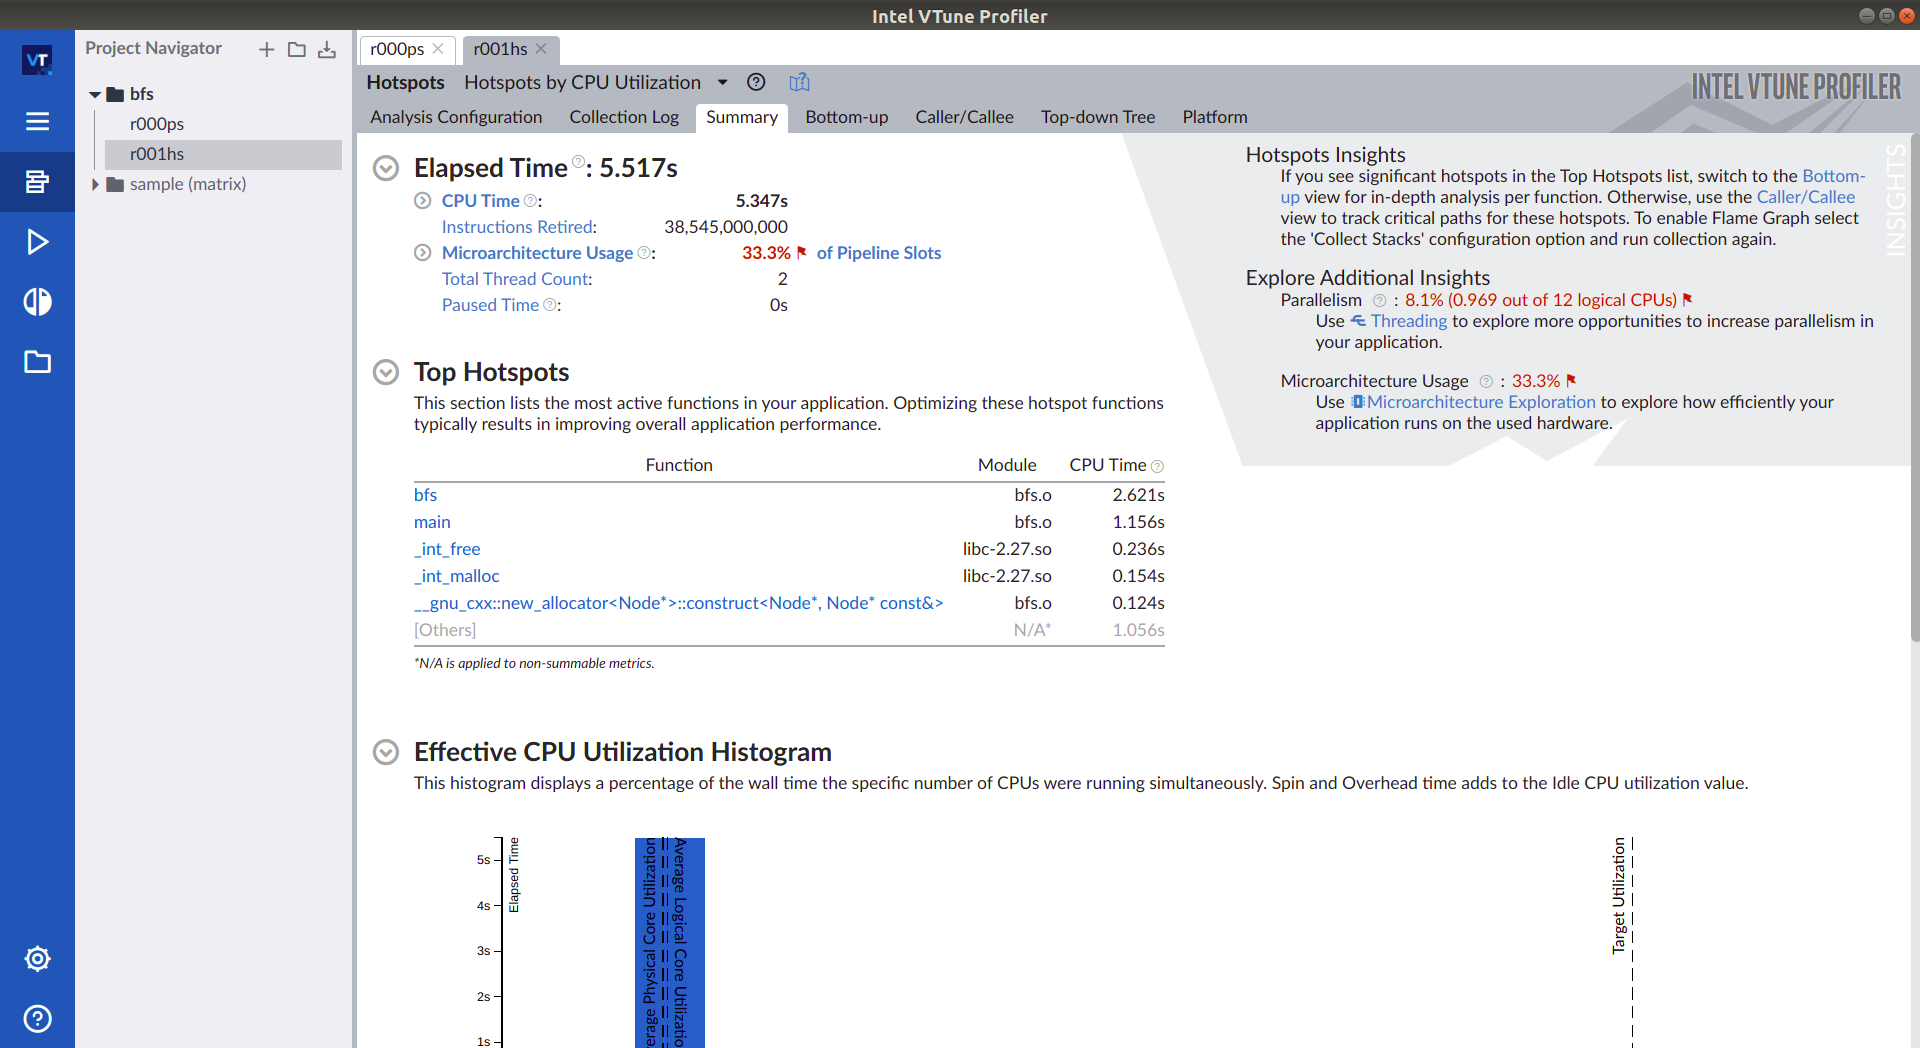
\includegraphics[scale=0.25]{vtune/bfs/hs.png}
    \caption{Top Functions by CPU Time for \texttt{bfs.cpp}}
\end{figure}

\newpage
\subsection*{Top 5 Source lines by CPU Utilization}
\begin{table}[H]
    \begin{tabular}{||l|l||c||}
        \hline
        Source                                               & Function                             & CPU Utilization \\
        \hline
        \texttt{if (left\_child) node\_Q.push(left\_child);} & \texttt{inline void bfs(Node *root)} & 22.7\%          \\
        \texttt{bfs(root);}                                  & \texttt{int main()}                  & 21.6\%          \\
        \texttt{right\_child = curr\_node->right;}           & \texttt{inline void bfs(Node *root)} & 17.2\%          \\
        \texttt{for (int i = 0; i < q\_size; i++) \{}        & \texttt{inline void bfs(Node *root)} & 4.8\%           \\
        \texttt{left\_child = curr\_node->left;}             & \texttt{inline void bfs(Node *root)} & 3.2\%           \\
        \hline
    \end{tabular}
\end{table}

\begin{figure}[H]
    \centering
    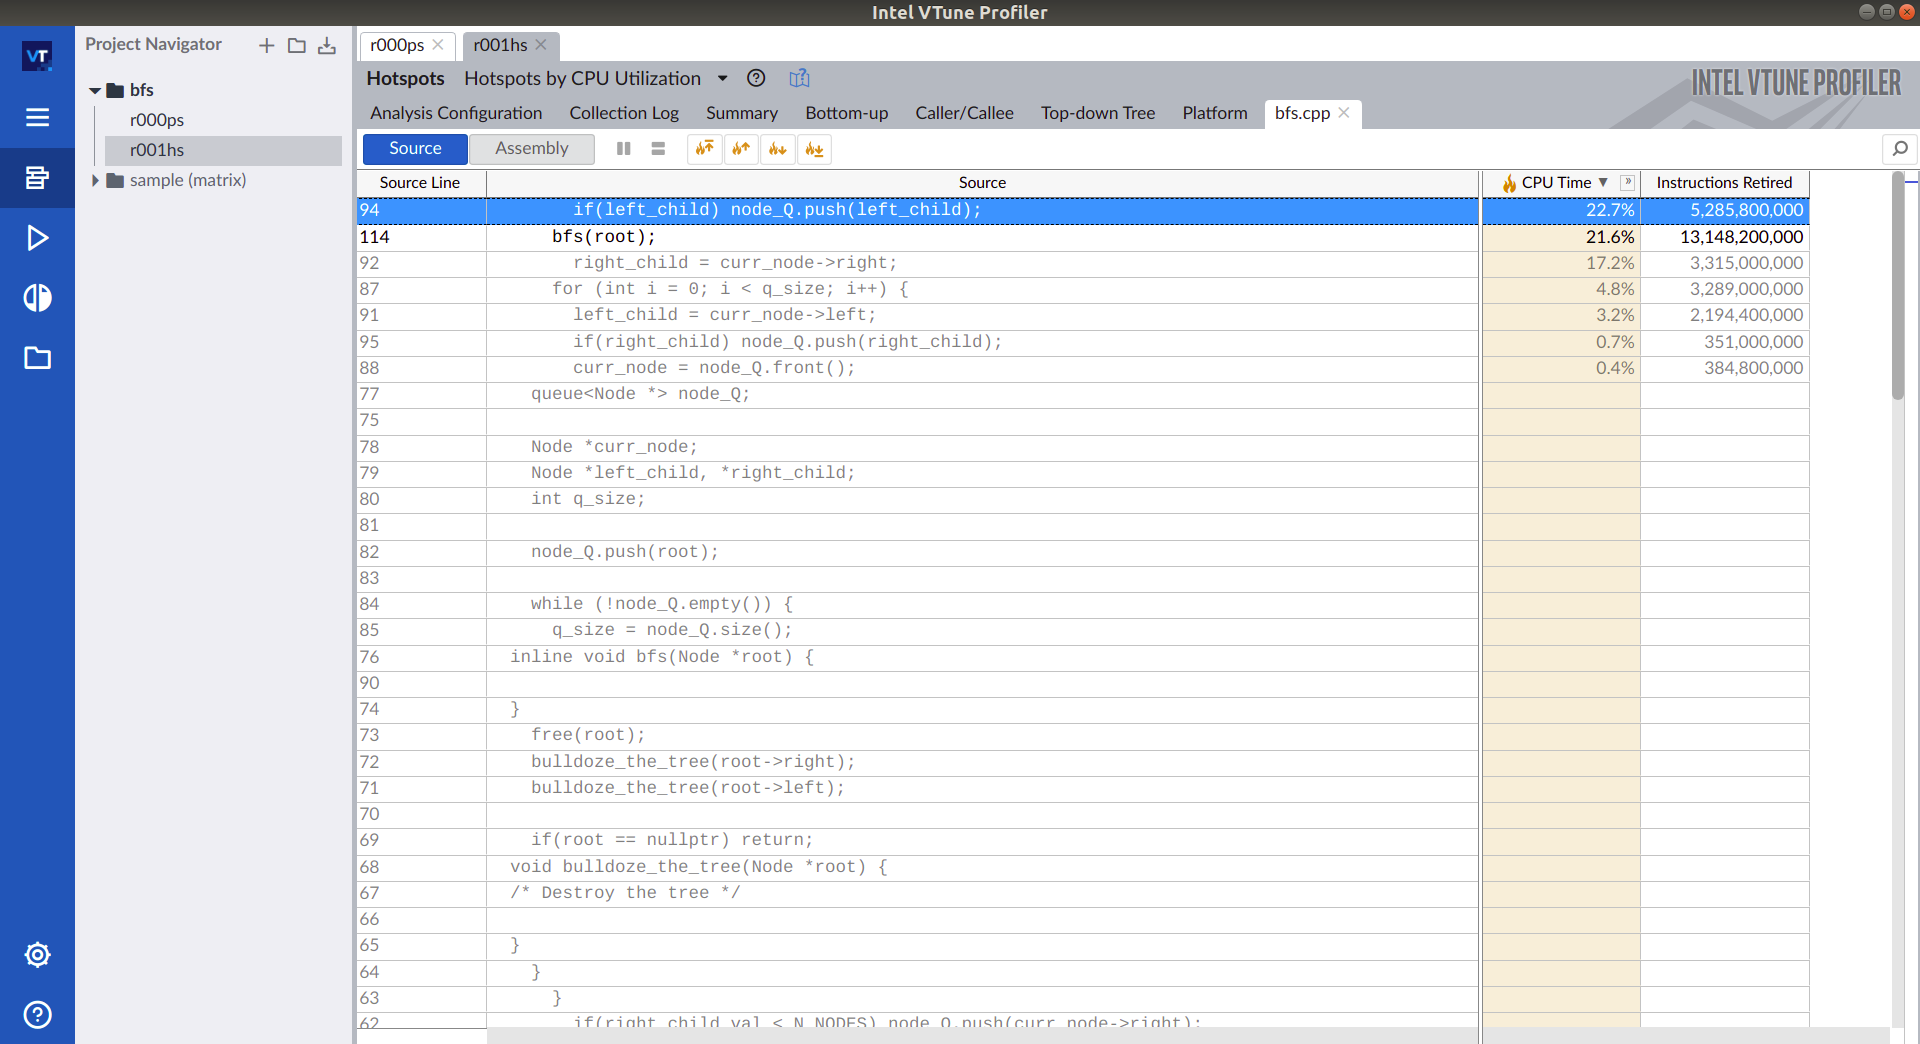
\includegraphics[scale=0.25]{vtune/bfs/sc.png}
    \caption{Top Source lines by CPU Utilization for \texttt{bfs.cpp}}
\end{figure}

\subsection*{Inference}
We see that majority of the time goes in function \texttt{bfs}.

The time consuming line in \texttt{main} is calling \texttt{bfs(root)}. This would be due to the need to set the function stack and as it is done for \texttt{N\_LOOPS} times, it climbs above \texttt{plant\_a\_tree} and \texttt{bulldoze\_the\_tree} stack setup.

Every line in \texttt{bfs} is called repeatedly due to 3 level of loops (2 level in \texttt{bfs} and 1 level in \texttt{main}). \\
These lines combined consume the majority of CPU time (\~50\%).


\newpage
\section{\texttt{matrix\_multi.cpp}}

\subsection*{Performance Snapshot}
\begin{itemize}
    \item IPC: 0.874
    \item Logical Core Utilization: 8.2\% (0.982 out of 12)
    \item Physical Core Utilization: 16.3\% (0.976 of 6)
    \item Memory bound: 59.1\% of Pipeline slots
\end{itemize}

\begin{figure}[H]
    \centering
    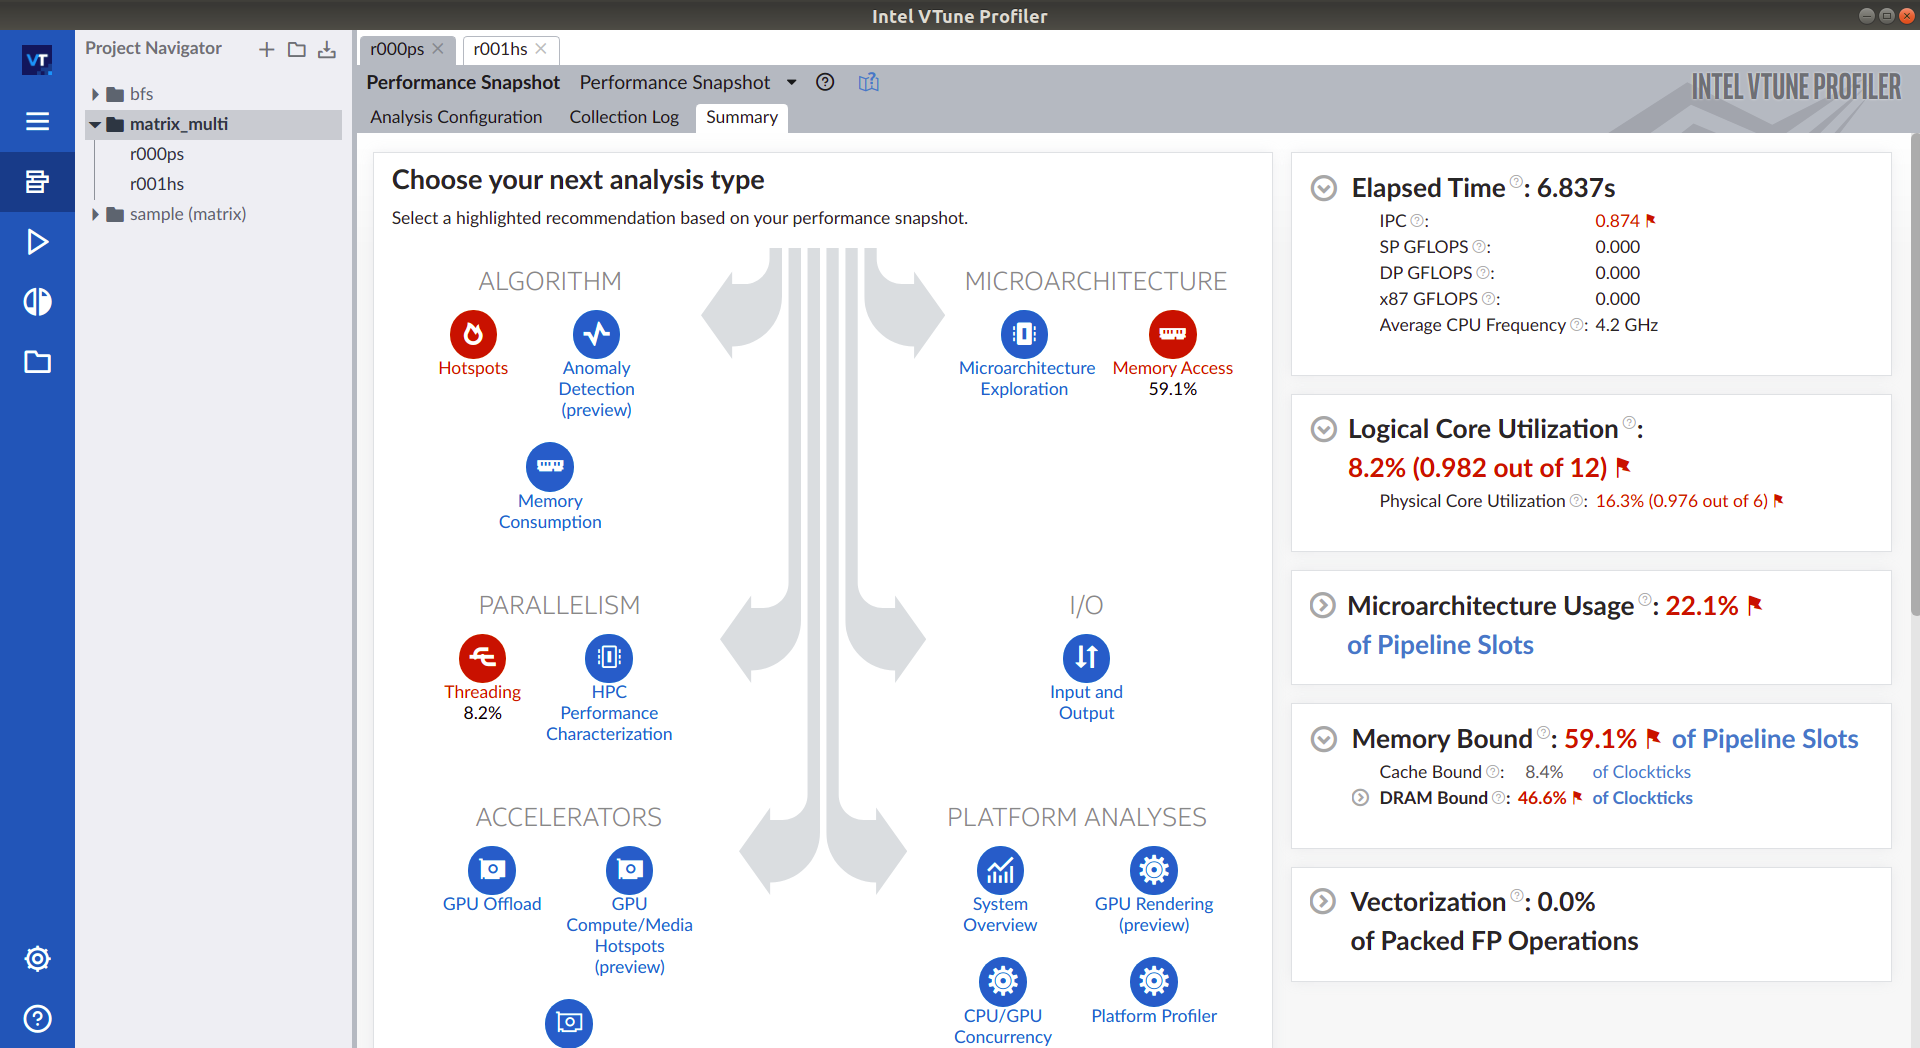
\includegraphics[scale=0.25]{vtune/matrix_multi/ps.png}
    \caption{Performance Snapshot for \texttt{matrix\_multi.cpp}}
\end{figure}

\newpage
\subsection*{Top Functions by CPU Time}
\begin{table}[H]
    \begin{tabular}{||l|l||c||}
        \hline
        Function                 & Module                   & CPU Time \\
        \hline
        \texttt{matrix\_product} & \texttt{matrix\_multi.o} & 6.597s   \\
        \hline
    \end{tabular}
\end{table}

\begin{figure}[H]
    \centering
    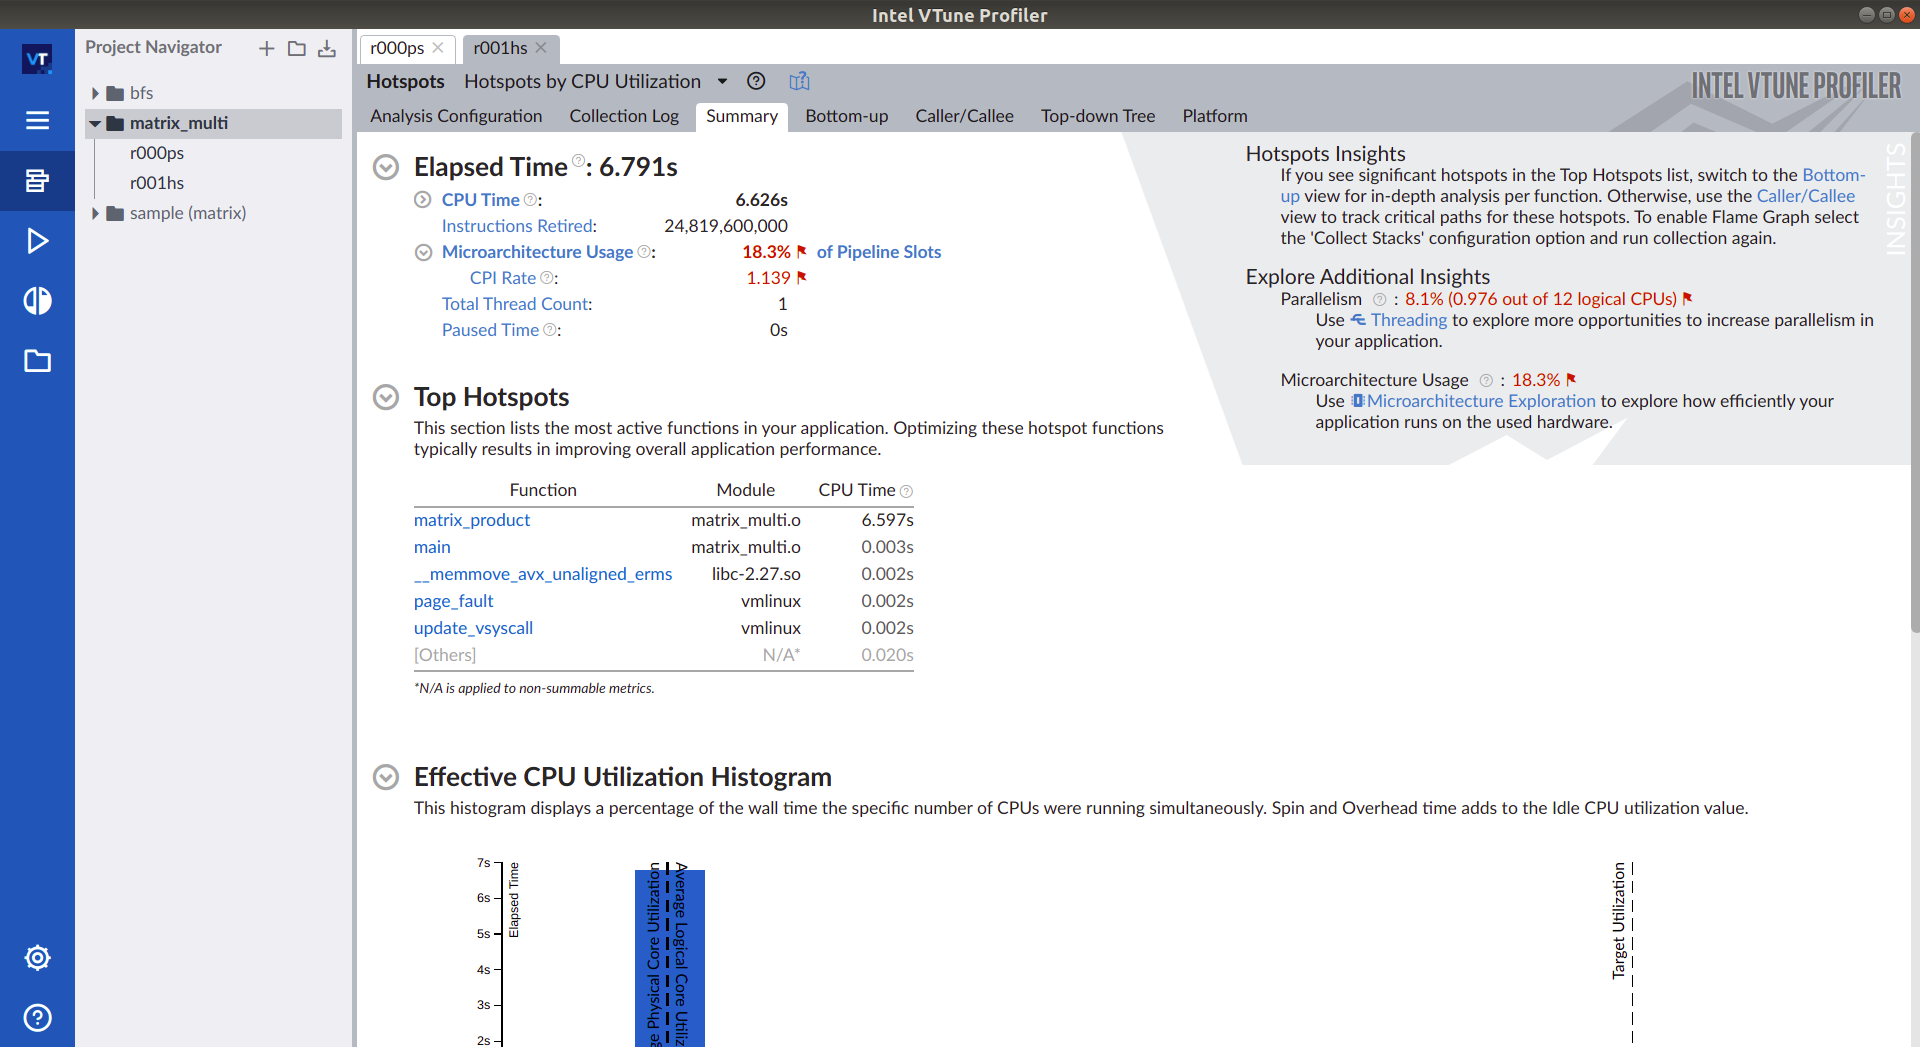
\includegraphics[scale=0.25]{vtune/matrix_multi/hs.png}
    \caption{Top Functions by CPU Time for \texttt{matrix\_multi.cpp}}
\end{figure}

\newpage
\subsection*{Top 2 Source lines by CPU Utilization}
\begin{table}[H]
    \begin{tabular}{||l|l||c||}
        \hline
        Source                                        & Function                        & CPU Utilization \\
        \hline
        \texttt{C[i][j] += A[i][k] * B[k][j];}        & \texttt{void matrix\_product()} & 90.9\%          \\
        \texttt{for (int k = 0; k < N\_DIMS; k++) \{} & \texttt{void matrix\_product()} & 8.6\%           \\
        \hline
    \end{tabular}
\end{table}

\begin{figure}[H]
    \centering
    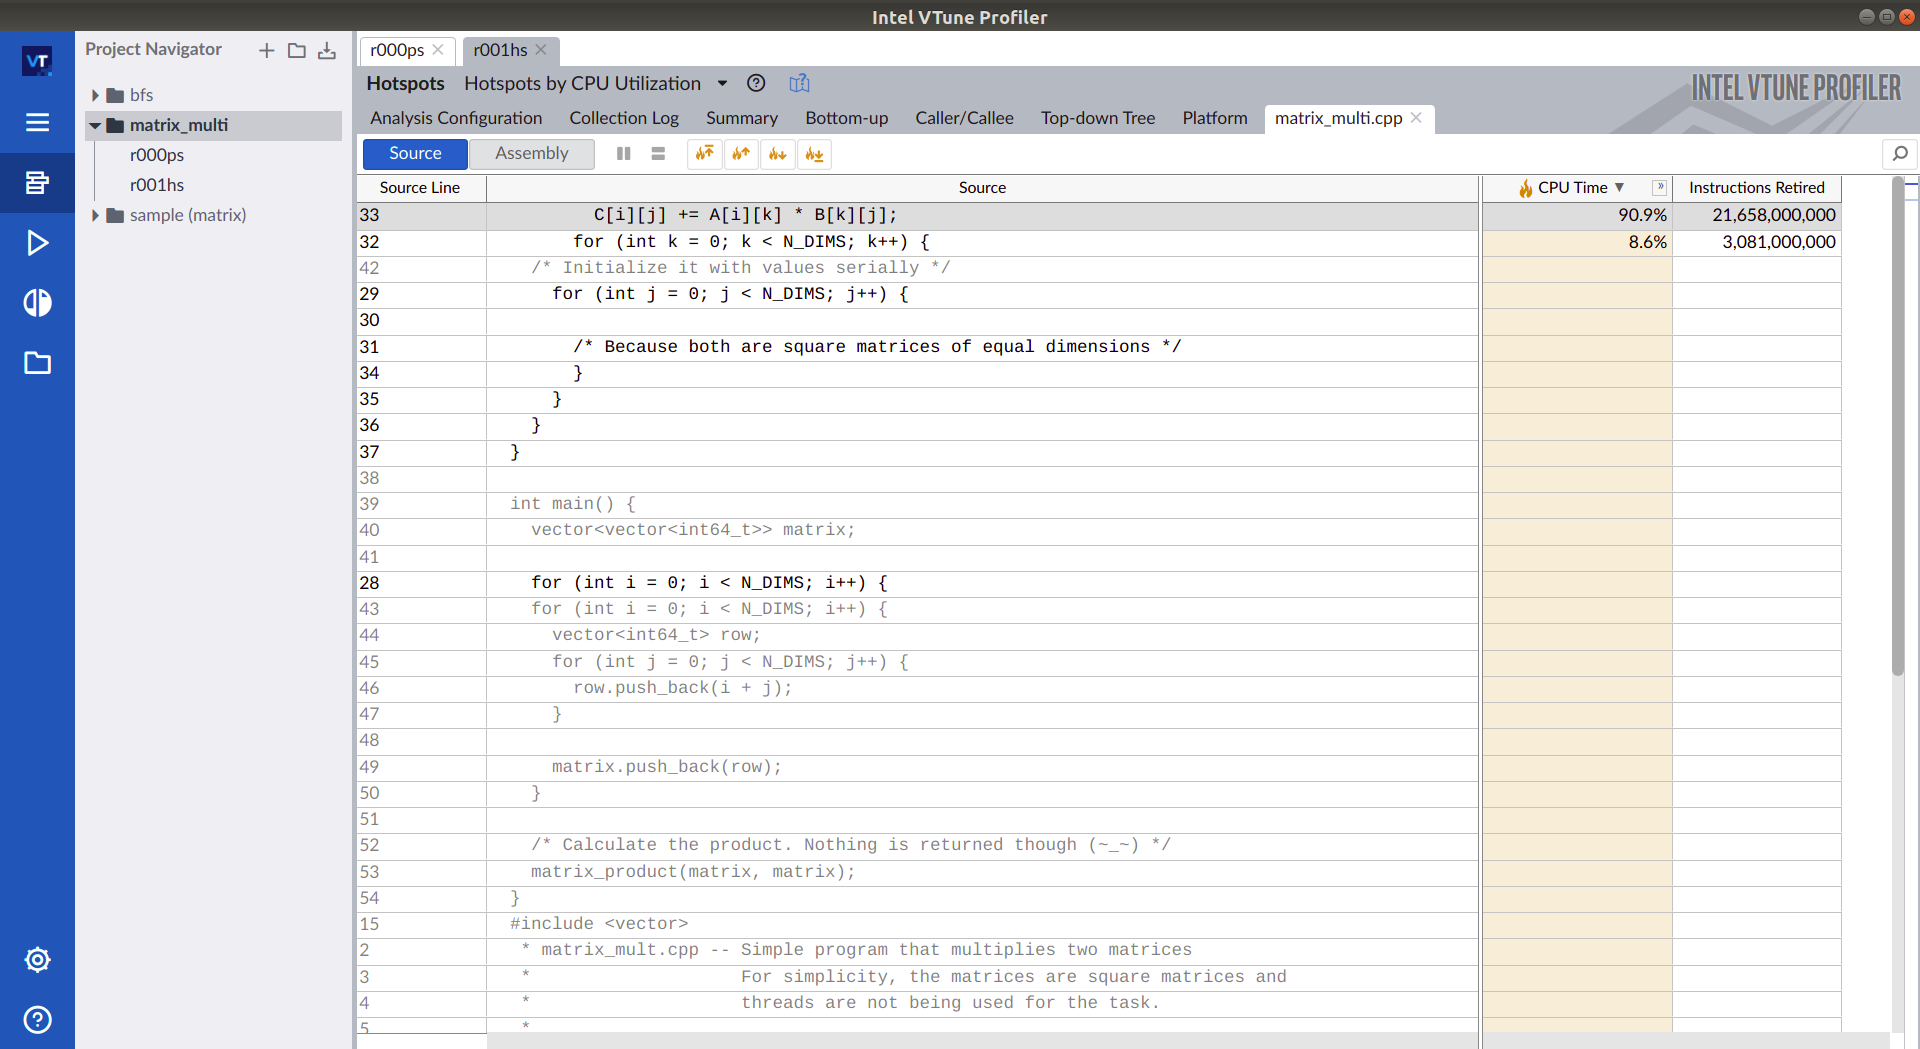
\includegraphics[scale=0.25]{vtune/matrix_multi/sc.png}
    \caption{Top Source lines by CPU Utilization for \texttt{matrix\_multi.cpp}}
\end{figure}

\subsection*{Inference}
We see that majority of the time goes in function \texttt{matrix\_product}.

As discussed in lectures, \texttt{ijk} is not the optimal loop order for memory access. We see that the inner loop takes most of the time. \\
And we access and modify \texttt{k} at every iteration of the inner loop, it is the line to take second most CPU time.


\newpage
\section{\texttt{matrix\_multi\_2.cpp}}

\subsection*{Performance Snapshot}
\begin{itemize}
    \item IPC: 1.339
    \item Logical Core Utilization: 8.2\% (0.981 out of 12)
    \item Physical Core Utilization: 16.2\% (0.973 of 6)
    \item Memory bound: 38.0\% of Pipeline slots
\end{itemize}

\begin{figure}[H]
    \centering
    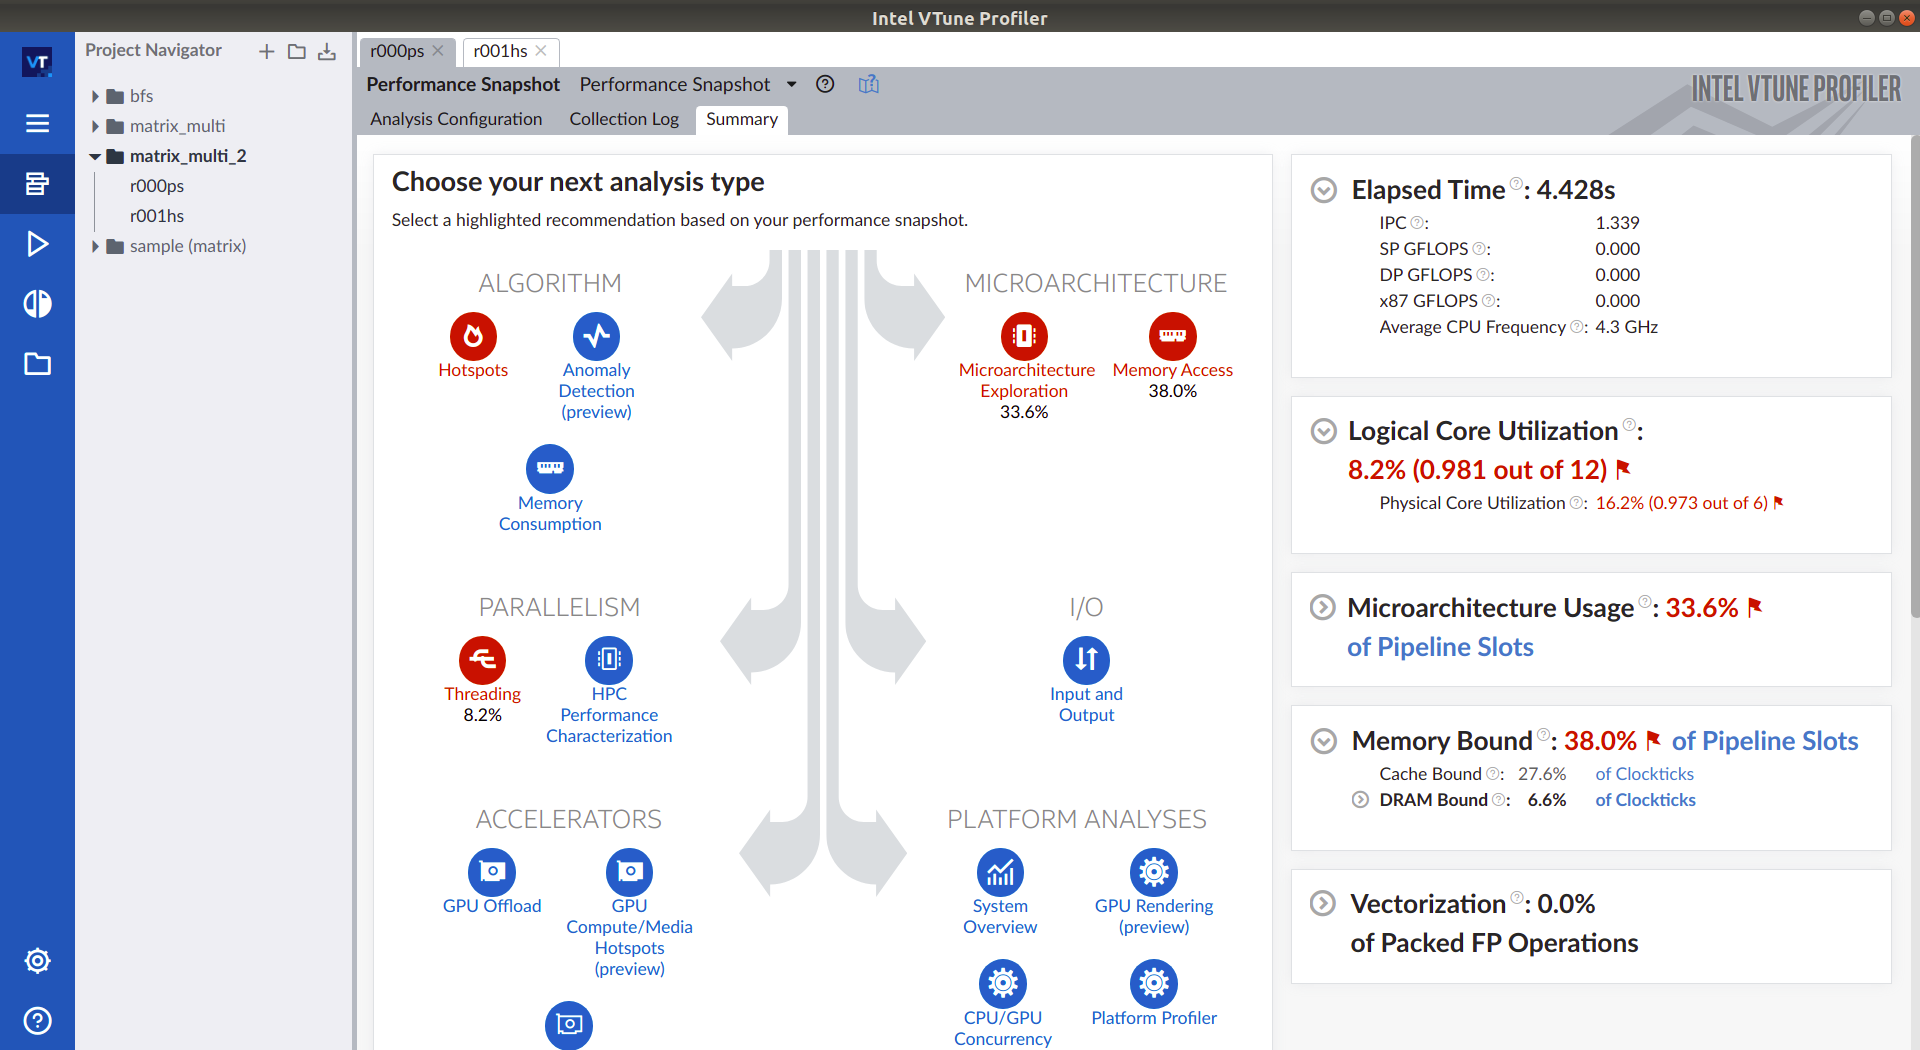
\includegraphics[scale=0.25]{vtune/matrix_multi_2/ps.png}
    \caption{Performance Snapshot for \texttt{matrix\_multi\_2.cpp}}
\end{figure}

\newpage
\subsection*{Top Functions by CPU Time}
\begin{table}[H]
    \begin{tabular}{||l|l||c||}
        \hline
        Function                 & Module                      & CPU Time \\
        \hline
        \texttt{matrix\_product} & \texttt{matrix\_multi\_2.o} & 4.492s   \\
        \hline
    \end{tabular}
\end{table}

\begin{figure}[H]
    \centering
    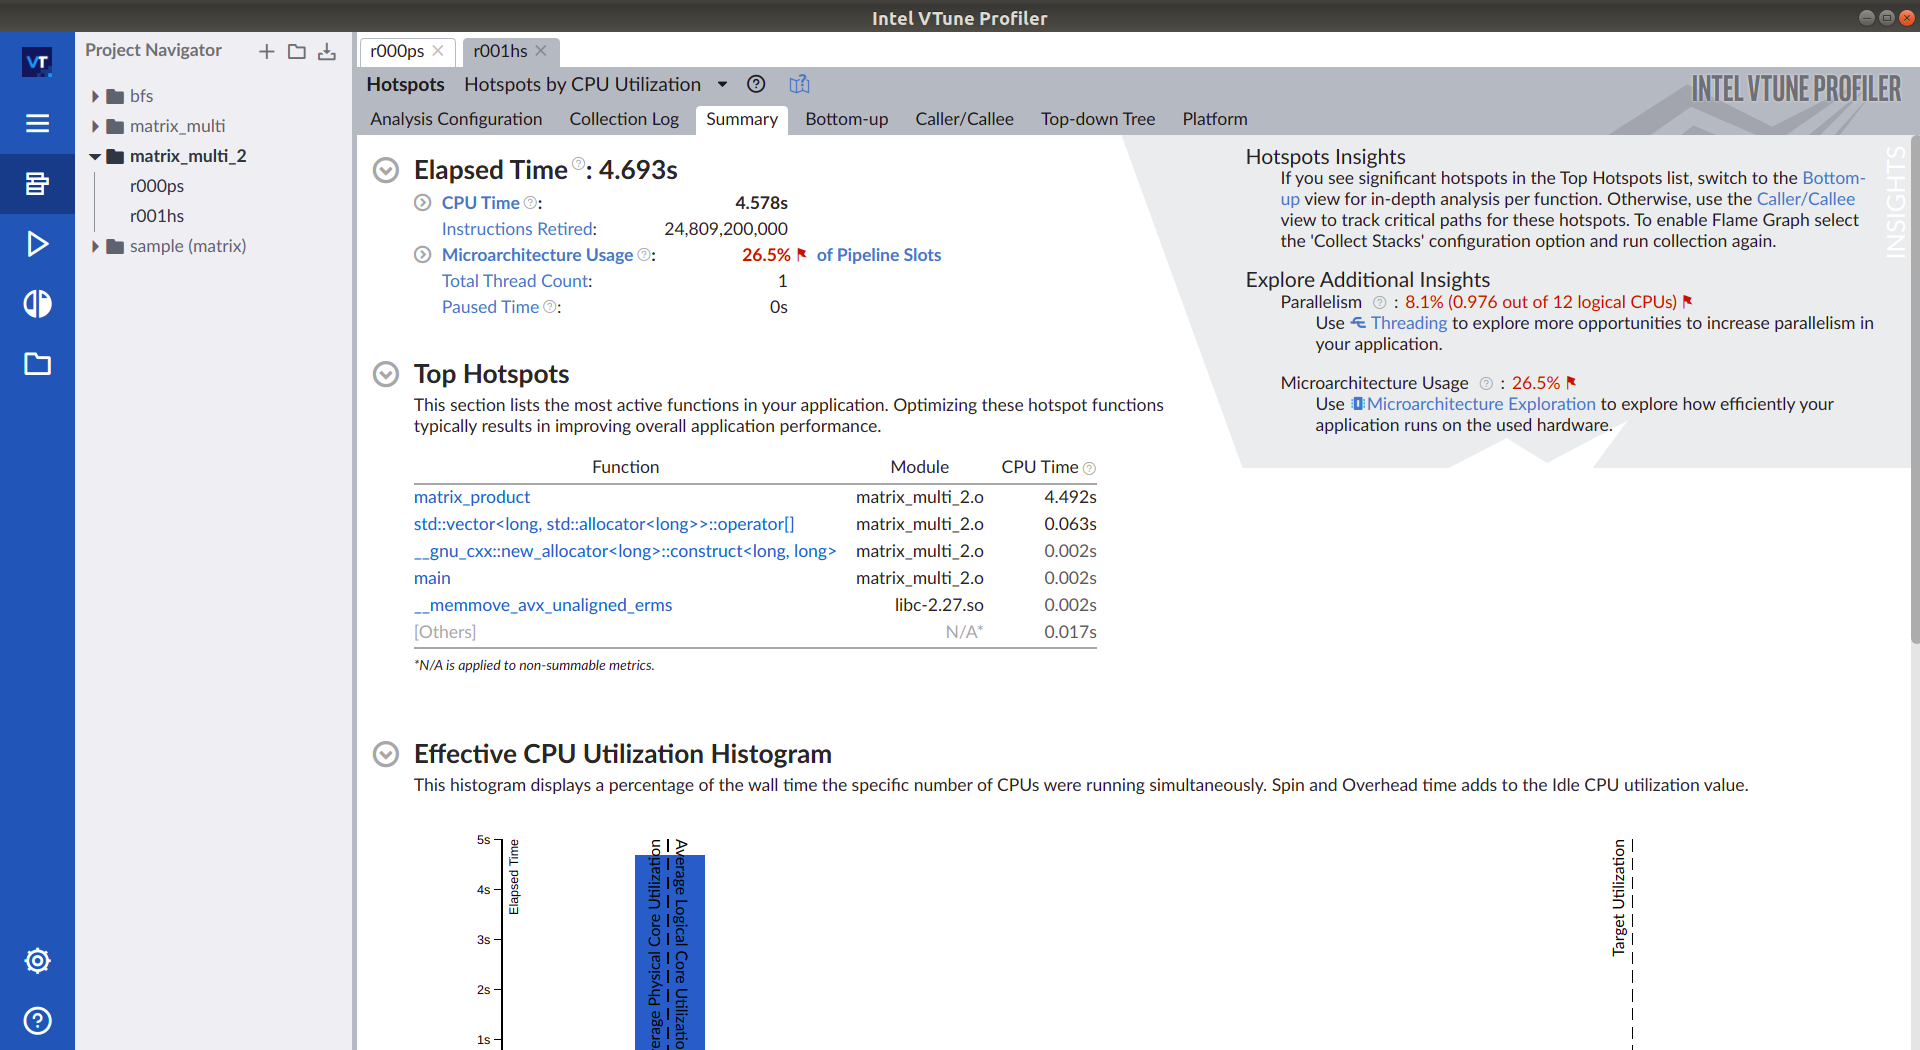
\includegraphics[scale=0.25]{vtune/matrix_multi_2/hs.png}
    \caption{Top Functions by CPU Time for \texttt{matrix\_multi\_2.cpp}}
\end{figure}

\newpage
\subsection*{Top 2 Source lines by CPU Utilization}
\begin{table}[H]
    \begin{tabular}{||l|l||c||}
        \hline
        Source                                        & Function                        & CPU Utilization \\
        \hline
        \texttt{C[i][j] += A[i][k] * B[k][j];}        & \texttt{void matrix\_product()} & 84.4\%          \\
        \texttt{for (int k = 0; k < N\_DIMS; k++) \{} & \texttt{void matrix\_product()} & 13.7\%          \\
        \hline
    \end{tabular}
\end{table}

\begin{figure}[H]
    \centering
    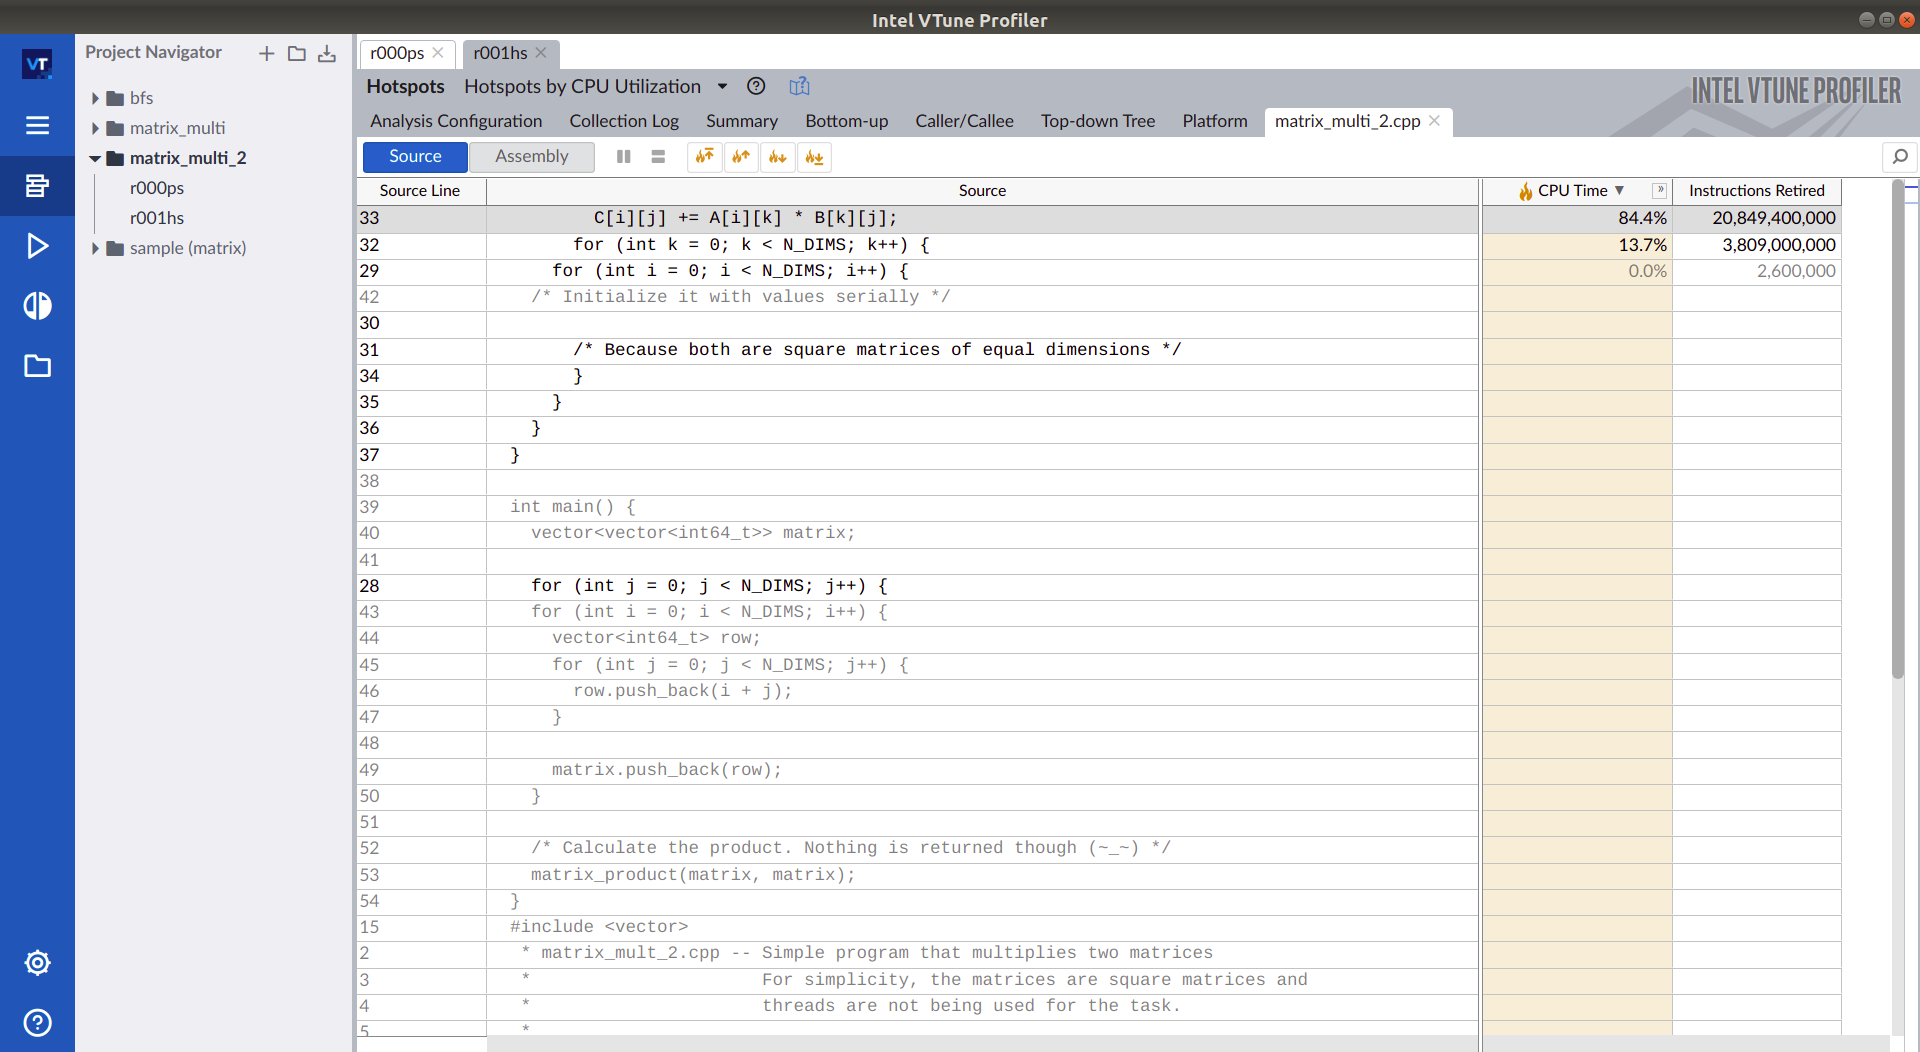
\includegraphics[scale=0.25]{vtune/matrix_multi_2/sc.png}
    \caption{Top Source lines by CPU Utilization for \texttt{matrix\_multi\_2.cpp}}
\end{figure}

\subsection*{Inference}
We see that majority of the time goes in function \texttt{matrix\_product}.

As discussed in lectures, \texttt{jik} (same as \texttt{ijk}) is not the optimal loop order for memory access. We see that the inner loop takes most of the time. \\
And we access and modify \texttt{k} at every iteration of the inner loop, it is the line to take second most CPU time.


\newpage
\section{\texttt{quicksort.cpp}}

\subsection*{Performance Snapshot}
\begin{itemize}
    \item IPC: 0.748
    \item Logical Core Utilization: 8.0\% (0.966 out of 12)
    \item Physical Core Utilization: 15.7\% (0.941 of 6)
    \item Memory bound: 23.0\% of Pipeline slots
\end{itemize}

\begin{figure}[H]
    \centering
    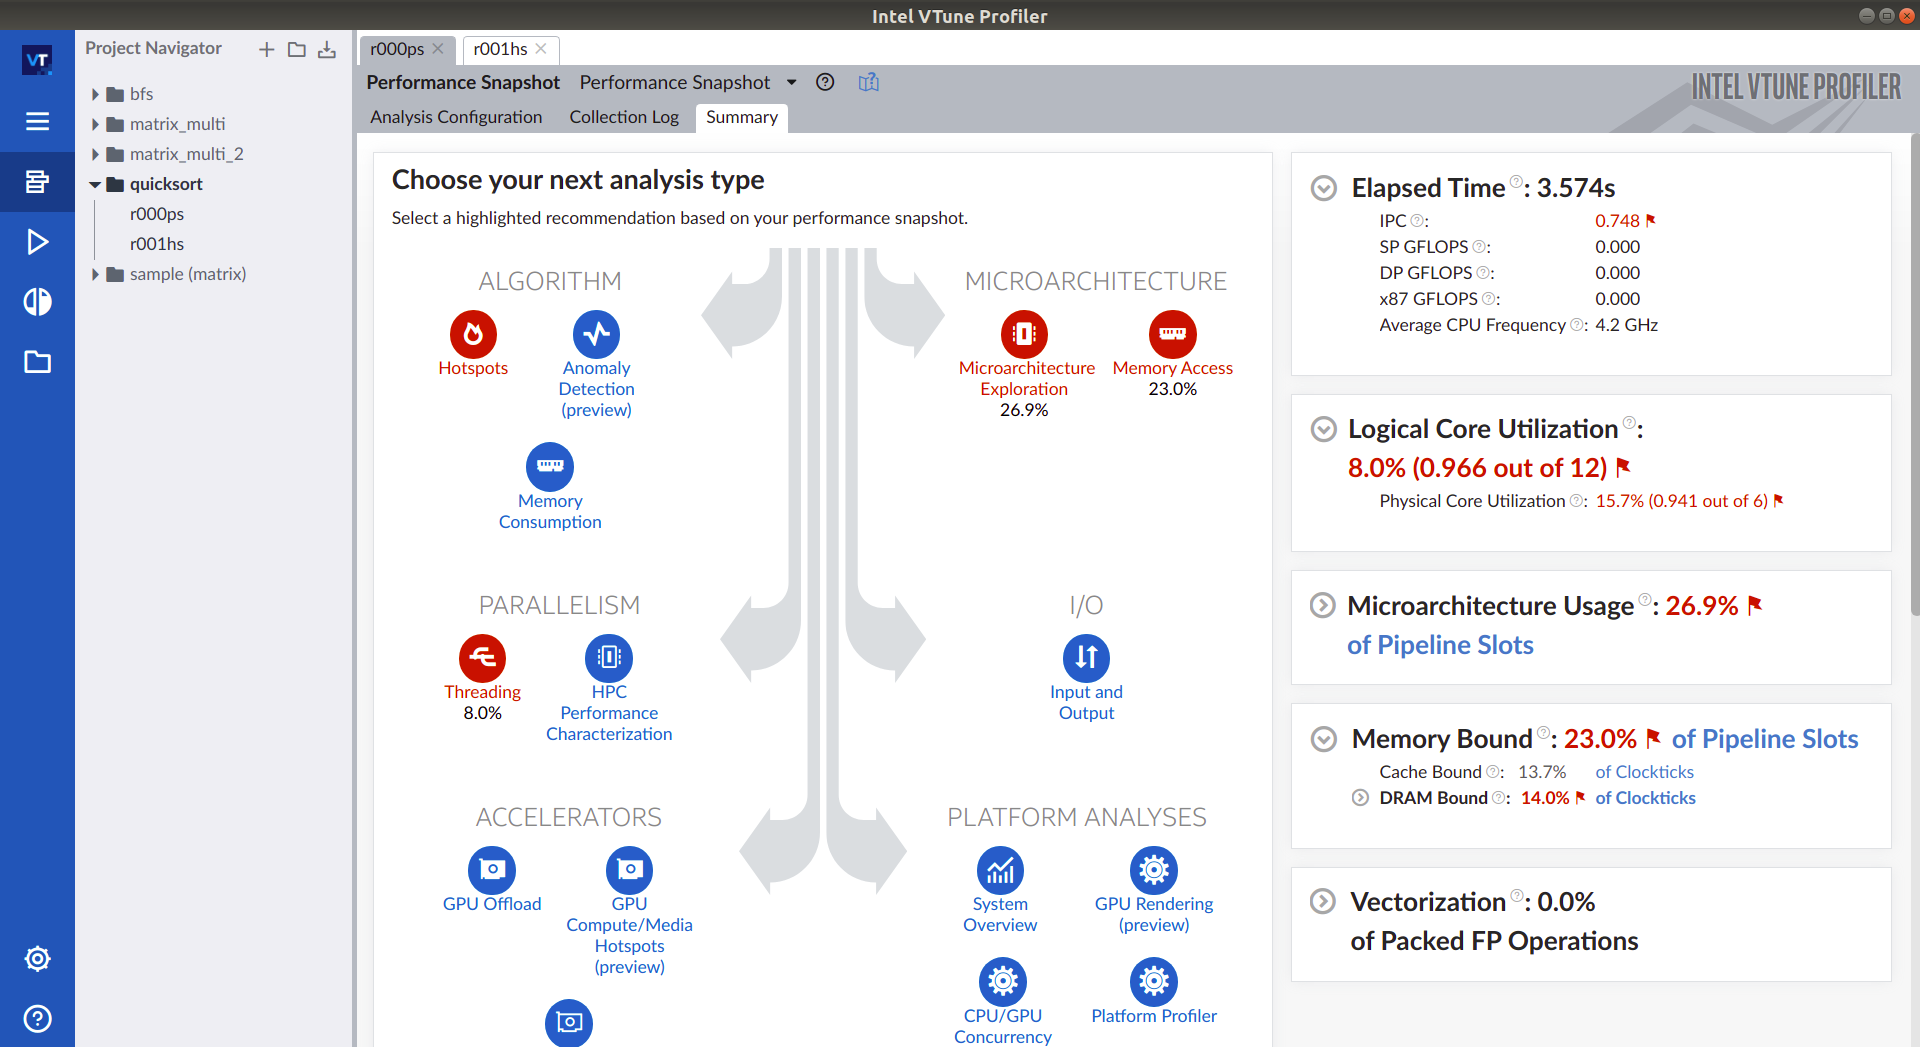
\includegraphics[scale=0.25]{vtune/quicksort/ps.png}
    \caption{Performance Snapshot for \texttt{quicksort.cpp}}
\end{figure}

\newpage
\subsection*{Top Functions by CPU Time}
\begin{table}[H]
    \begin{tabular}{||l|l||c||}
        \hline
        Function                                   & Module                & CPU Time \\
        \hline
        \texttt{\_\_memmove\_avx\_unaligned\_erms} & \texttt{libc-2.27.so} & 0.875s   \\
        \texttt{page\_fault}                       & \texttt{vmlinux}      & 0.511s   \\
        \texttt{clear\_page\_erms}                 & \texttt{vmlinux}      & 0.228s   \\
        \texttt{prepare\_exit\_to\_usermode}       & \texttt{vmlinux}      & 0.226s   \\
        \texttt{perf\_iterate\_ctx}                & \texttt{vmlinux}      & 0.155s   \\
        Others                                     & N/A                   & 1.545s   \\
        \hline
    \end{tabular}
\end{table}

\begin{figure}[H]
    \centering
    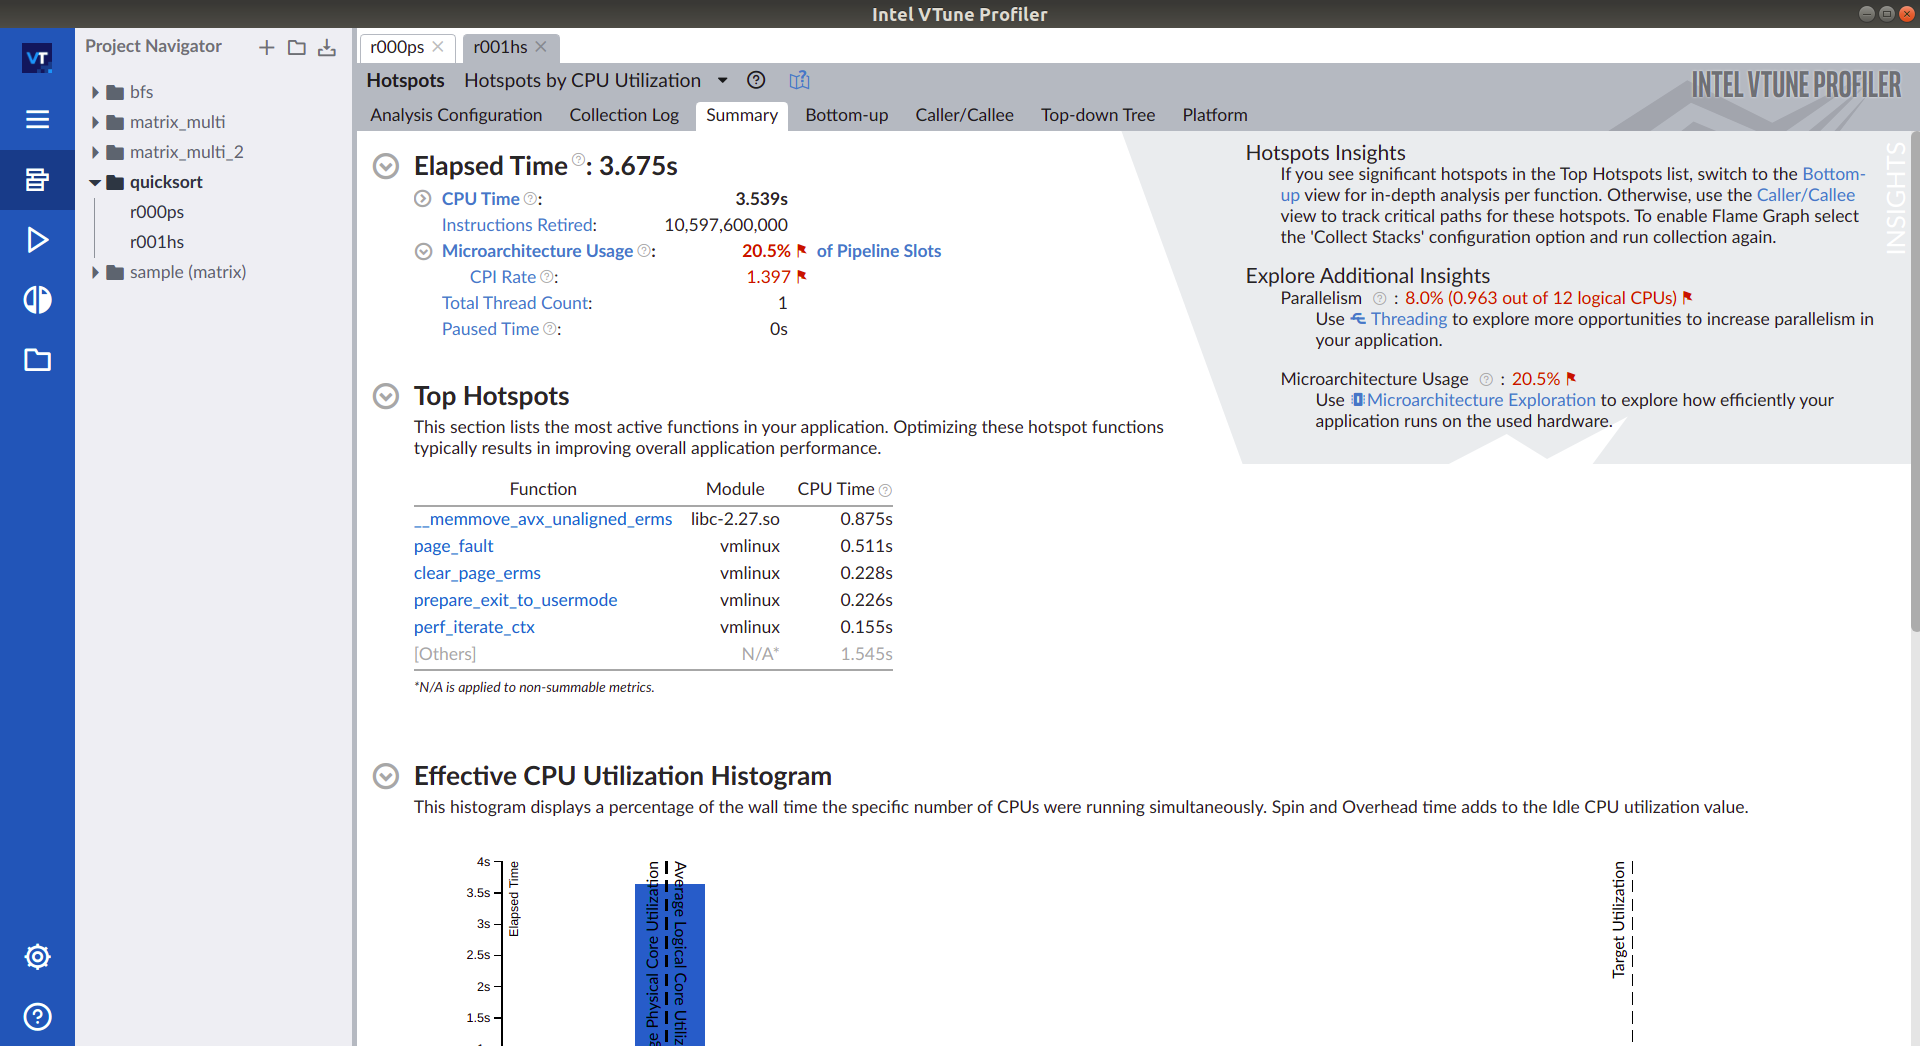
\includegraphics[scale=0.25]{vtune/quicksort/hs.png}
    \caption{Top Functions by CPU Time for \texttt{quicksort.cpp}}
\end{figure}

\newpage
\subsection*{Top 5 Source lines by CPU Utilization}
\begin{table}[H]
    \begin{tabular}{||l|l||c||}
        \hline
        Source                                     & Function                  & CPU Utilization \\
        \hline
        \texttt{b = c;}                            & \texttt{void swap()}      & 2.1\%           \\
        \texttt{if (nums[i] < pivot) \{}           & \texttt{long partition()} & 1.9\%           \\
        \texttt{slow\_ptr++;}                      & \texttt{long partition()} & 1.7\%           \\
        \texttt{for (long i = lo; i < hi; i++) \{} & \texttt{long partition()} & 0.6\%           \\
        \texttt{a = b;}                            & \texttt{void swap()}      & 0.2\%           \\
        \hline
    \end{tabular}
\end{table}

\begin{figure}[H]
    \centering
    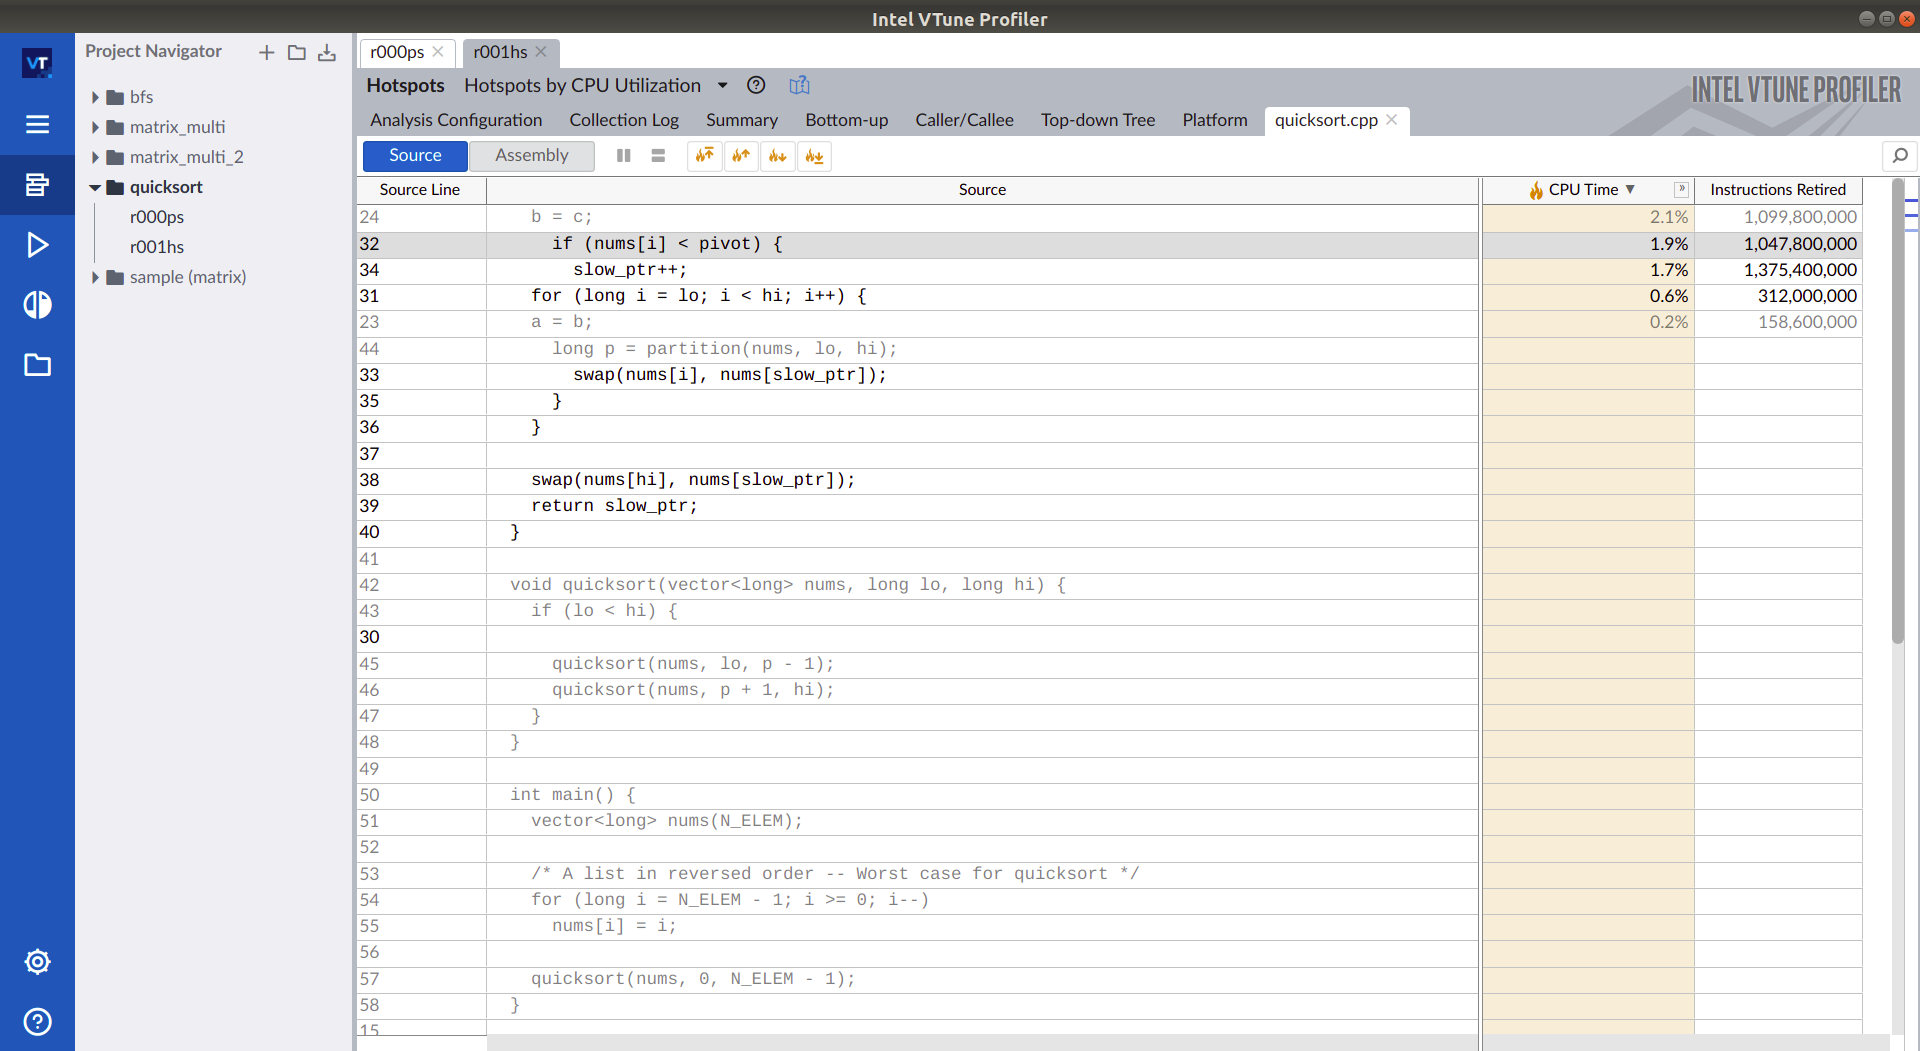
\includegraphics[scale=0.25]{vtune/quicksort/sc.png}
    \caption{Top Source lines by CPU Utilization for \texttt{quicksort.cpp}}
\end{figure}

\subsection*{Inference}
We see that majority of the time goes in handling page faults and \texttt{memmove}. Possible explanation is that because it crosses my limit of RAM and overflows in swap memory, we might be getting page faults and page needs to be loaded back from the swap memory. (We discussed this in OS course)

The lines (present in \texttt{quicksort.cpp}) consuming the majority of time is mostly because of the number of times it is executed. \\
Quicksort algorithm is mostly partitioning and swapping, so those two functions take the majority of the time.


%%%%%%%%%%%%%%%%%%%%%%%%%%%%%%%%%%%%%%%%%%%%%%%%
%% Part 2: Simulating with ChampSim
%%%%%%%%%%%%%%%%%%%%%%%%%%%%%%%%%%%%%%%%%%%%%%%%
\chapter{Simulating with ChampSim}
\section{Prepare traces}

Generate tracer for champsim: \\
\texttt{cd /champsim/ChampSim/tracer; ./make\_tracer.sh;} \\
Used pin to generate traces: \\
\texttt{pin -t obj-intel64/champsim\_tracer.so -o <program>.trace -t 21000000 -- <executable>;} \\
Used xz to compress the traces: \\
\texttt{xz -vz <program>.trace --threads=0;}

\begin{table}[H]
    \begin{tabular}{||c||c|c||c||}
        \hline
        Program                     & Parameters                                         & Execution time & Trace size \\
        \hline
        \texttt{bfs.o}              & \texttt{N\_NODES (1<<15)}; \texttt{N\_LOOPS 1000}; & 3.4 s          & 2092 KB    \\
        \hline
        \texttt{matrix\_multi.o}    & \texttt{N\_DIMS 700};                              & 4.5 s          & 2172 KB    \\
        \hline
        \texttt{matrix\_multi\_2.o} & \texttt{N\_DIMS 700};                              & 4.2 s          & 2160 KB    \\
        \hline
        \texttt{quicksort.o}        & \texttt{N\_ELEM (1<<14)};                          & 3.1 s          & 4172 KB    \\
        \hline
    \end{tabular}
\end{table}

\section{Setup Configurations}

To speed up the task and to avoid having to reset to default values again and again, I prepared 7 copies of ChampSim in the docker container. \\
This helped me run the 28 simulations in parallel and the entire experiment took 5-6 minutes to finish.

To setup each of the Configurations, I had to modify \texttt{./inc/cache.h}.

I have used \hyperlink{https://github.com/HewlettPackard/cacti}{CACTI} to compute the latency updates for changes in cache size. \\
Theoretically, there would be change in latency when we change associativity as well but as it wasn't present in PS I have ignored it. \\
As hinted by professor, latency of 12-way cache is computed by taking mean of latency of 8-way and 16-way caches keeping sets as constant. \\
For \texttt{L1I} and \texttt{L1D} caches, the change in access time was small, so the latency remains same across the configurations. \\
Also, I have rounded off the latency to nearest integers to avoid issues with ChampSim. \\
(For example, I got \texttt{L1I\_LATENCY} to be 3.8 and 4.2 for half and double size cache respectively. I have consider both of them as 4 - same as baseline) \\


\newpage
\subsection*{Updates in \texttt{./inc/cache.h}}
\begin{table}[H]
    \begin{tabular}{||c|c||c||c|c||c|c||c|c||}
        \hline
        \multirow{2}{*}{Line} & \multirow{2}{*}{Parameter} & \multirow{2}{*}{Baseline} & Direct  & Fully       & Reduced & Doubled & Reduced & Doubled \\
                              &                            &                           & Mapped  & Associative & Size    & Size    & MSHR    & MSHR    \\
        \hline
        46                    & \texttt{L1I\_SET}          & 64                        & 64*8    & 1           & 32      & 128     & 64      & 64      \\
        47                    & \texttt{L1I\_WAY}          & 8                         & 1       & 8*64        & 8       & 8       & 8       & 8       \\
        51                    & \texttt{L1I\_MSHR\_SIZE}   & 8                         & 8       & 8           & 8       & 8       & 4       & 16      \\
        52                    & \texttt{L1I\_LATENCY}      & 4                         & 4       & 4           & 4       & 4       & 4       & 4       \\
        \hline
        55                    & \texttt{L1D\_SET}          & 64                        & 64*12   & 1           & 32      & 128     & 64      & 64      \\
        56                    & \texttt{L1D\_WAY}          & 12                        & 1       & 12*64       & 12      & 12      & 12      & 12      \\
        60                    & \texttt{L1D\_MSHR\_SIZE}   & 16                        & 16      & 16          & 16      & 16      & 8       & 32      \\
        61                    & \texttt{L1D\_LATENCY}      & 5                         & 5       & 5           & 5       & 5       & 5       & 5       \\
        \hline
        64                    & \texttt{L2C\_SET}          & 1024                      & 1024*8  & 1           & 512     & 2048    & 1024    & 1024    \\
        65                    & \texttt{L2C\_WAY}          & 8                         & 1       & 8*1024      & 8       & 8       & 8       & 8       \\
        69                    & \texttt{L2C\_MSHR\_SIZE}   & 32                        & 32      & 32          & 32      & 32      & 16      & 64      \\
        70                    & \texttt{L2C\_LATENCY}      & 10                        & 10      & 10          & 9       & 13      & 10      & 10      \\
        \hline
        73                    & \texttt{LLC\_SET}          & 2048                      & 2048*16 & 1           & 1024    & 4096    & 2048    & 2048    \\
        74                    & \texttt{LLC\_WAY}          & 16                        & 1       & 16*2048     & 16      & 16      & 16      & 16      \\
        78                    & \texttt{LLC\_MSHR\_SIZE}   & 64                        & 64      & 64          & 64      & 64      & 32      & 128     \\
        79                    & \texttt{LLC\_LATENCY}      & 20                        & 20      & 20          & 17      & 24      & 20      & 20      \\
        \hline
    \end{tabular}
\end{table}


\section{\texttt{bfs.trace.xz}}
\begin{table}[H]
    \begin{tabular}{||c|c||c||c|c||c|c||c|c||}
        \hline
        \multicolumn{2}{||c||}{\multirow{2}{*}{Parameter}} & \multirow{2}{*}{Baseline} & Direct   & Fully       & Reduced  & Doubled  & Reduced  & Doubled  \\
        \multicolumn{2}{||c||}{}                           &                           & Mapped   & Associative & Size     & Size     & MSHR     & MSHR     \\
        \hline
        \multicolumn{2}{||c||}{cycles}                     & 11505060                  & 11548164 & 11510528    & 11646705 & 11410653 & 11505205 & 11504968 \\
        \multicolumn{2}{||c||}{IPC}                        & 0.869183                  & 0.865938 & 0.86877     & 0.858612 & 0.876374 & 0.869172 & 0.86919  \\
        \hline
                                            & \texttt{L1D} & 21942                     & 30732    & 21942       & 21947    & 21931    & 21942    & 21972    \\
        Cache                               & \texttt{L1I} & 1                         & 201163   & 1           & 9        & 1        & 1        & 1        \\
        Misses                              & \texttt{L2C} & 21464                     & 23645    & 21727       & 21881    & 14648    & 21464    & 21464    \\
                                            & \texttt{LLC} & 13437                     & 14032    & 13437       & 14920    & 13436    & 13437    & 13437    \\
        \hline
                                            & \texttt{L1D} & 2.1942                    & 3.0732   & 2.1942      & 2.1947   & 2.1931   & 2.1942   & 2.1972   \\
        \multirow{2}{*}{MPKI}               & \texttt{L1I} & 0.0001                    & 20.1163  & 0.0001      & 0.0009   & 0.0001   & 0.0001   & 0.0001   \\
                                            & \texttt{L2C} & 2.1464                    & 2.3645   & 2.1727      & 2.1881   & 1.4648   & 2.1464   & 2.1464   \\
                                            & \texttt{LLC} & 1.3437                    & 1.4032   & 1.3437      & 1.4920   & 1.3436   & 1.3437   & 1.3437   \\
        \hline
                                            & \texttt{L1D} & 91.8093                   & 71.4266  & 91.6041     & 130.174  & 85.5957  & 91.7903  & 91.844   \\
        Avg Miss                            & \texttt{L1I} & 215                       & 14.1125  & 215         & 57.6667  & 229      & 215      & 215      \\
        Latency                             & \texttt{L2C} & 78.5156                   & 73.5786  & 77.3577     & 116.525  & 107.193  & 78.4964  & 78.5508  \\
                                            & \texttt{LLC} & 77.5087                   & 79.0059  & 76.5858     & 132.767  & 76.5338  & 77.4779  & 77.5649  \\
        \hline
    \end{tabular}
\end{table}


\section{\texttt{matrix\_multi.trace.xz}}
\begin{table}[H]
    \begin{tabular}{||c|c||c||c|c||c|c||c|c||}
        \hline
        \multicolumn{2}{||c||}{\multirow{2}{*}{Parameter}} & \multirow{2}{*}{Baseline} & Direct   & Fully       & Reduced  & Doubled  & Reduced  & Doubled  \\
        \multicolumn{2}{||c||}{}                           &                           & Mapped   & Associative & Size     & Size     & MSHR     & MSHR     \\
        \hline
        \multicolumn{2}{||c||}{cycles}                     & 17624045                  & 17696897 & 17624045    & 17625492 & 17624129 & 17624452 & 17623986 \\
        \multicolumn{2}{||c||}{IPC}                        & 0.567407                  & 0.565071 & 0.567407    & 0.56736  & 0.567404 & 0.567394 & 0.567409 \\
        \hline
                                            & \texttt{L1D} & 7392                      & 20961    & 7393        & 9130     & 7381     & 7392     & 7392     \\
        Cache                               & \texttt{L1I} & 0                         & 8396     & 0           & 174      & 0        & 0        & 0        \\
        Misses                              & \texttt{L2C} & 7269                      & 7707     & 7269        & 7481     & 7268     & 7269     & 7269     \\
                                            & \texttt{LLC} & 7268                      & 7548     & 7268        & 7268     & 7268     & 7268     & 7268     \\
        \hline
                                            & \texttt{L1D} & 0.7392                    & 2.0961   & 0.7393      & 0.9130   & 0.7381   & 0.7392   & 0.7392   \\
        \multirow{2}{*}{MPKI}               & \texttt{L1I} & 0.0000                    & 0.8396   & 0.0000      & 0.0174   & 0.0000   & 0.0000   & 0.0000   \\
                                            & \texttt{L2C} & 0.7269                    & 0.7707   & 0.7269      & 0.7481   & 0.7268   & 0.7269   & 0.7269   \\
                                            & \texttt{LLC} & 0.7268                    & 0.7548   & 0.7268      & 0.7268   & 0.7268   & 0.7268   & 0.7268   \\
        \hline
                                            & \texttt{L1D} & 117.04                    & 52.756   & 117.026     & 101.301  & 130.94   & 116.558  & 118.607  \\
        Avg Miss                            & \texttt{L1I} & -                         & 14.2587  & -           & 20.1954  & -        & -        & -        \\
        Latency                             & \texttt{L2C} & 103.766                   & 103.328  & 103.766     & 106.711  & 114.666  & 103.277  & 105.36   \\
                                            & \texttt{LLC} & 73.7643                   & 76.0135  & 73.7643     & 83.4732  & 77.6564  & 73.275   & 75.3581  \\
        \hline
    \end{tabular}
\end{table}


\section{\texttt{matrix\_multi\_2.trace.xz}}
\begin{table}[H]
    \begin{tabular}{||c|c||c||c|c||c|c||c|c||}
        \hline
        \multicolumn{2}{||c||}{\multirow{2}{*}{Parameter}} & \multirow{2}{*}{Baseline} & Direct   & Fully       & Reduced  & Doubled  & Reduced  & Doubled  \\
        \multicolumn{2}{||c||}{}                           &                           & Mapped   & Associative & Size     & Size     & MSHR     & MSHR     \\
        \hline
        \multicolumn{2}{||c||}{cycles}                     & 17622240                  & 17694653 & 17622240    & 17623493 & 17622347 & 17622647 & 17622268 \\
        \multicolumn{2}{||c||}{IPC}                        & 0.567465                  & 0.565143 & 0.567465    & 0.567424 & 0.567461 & 0.567452 & 0.567464 \\
        \hline
                                            & \texttt{L1D} & 7392                      & 21323    & 7393        & 9140     & 7381     & 7392     & 7392     \\
        Cache                               & \texttt{L1I} & 0                         & 6867     & 0           & 174      & 0        & 0        & 0        \\
        Misses                              & \texttt{L2C} & 7269                      & 7857     & 7269        & 7483     & 7268     & 7269     & 7269     \\
                                            & \texttt{LLC} & 7268                      & 7465     & 7268        & 7268     & 7268     & 7268     & 7268     \\
        \hline
                                            & \texttt{L1D} & 0.7392                    & 2.1323   & 0.7393      & 0.9140   & 0.7381   & 0.7392   & 0.7392   \\
        \multirow{2}{*}{MPKI}               & \texttt{L1I} & 0.0000                    & 0.6867   & 0.0000      & 0.0174   & 0.0000   & 0.0000   & 0.0000   \\
                                            & \texttt{L2C} & 0.7269                    & 0.7857   & 0.7269      & 0.7483   & 0.7268   & 0.7269   & 0.7269   \\
                                            & \texttt{LLC} & 0.7268                    & 0.7645   & 0.7268      & 0.7268   & 0.7268   & 0.7268   & 0.7268   \\
        \hline
                                            & \texttt{L1D} & 116.464                   & 53.2717  & 116.329     & 101.704  & 130.203  & 116.168  & 117.712  \\
        Avg Miss                            & \texttt{L1I} & -                         & 14.8274  & -           & 19.4425  & -        & -        & -        \\
        Latency                             & \texttt{L2C} & 103.181                   & 105.285  & 103.057     & 107.273  & 113.948  & 102.88   & 104.45   \\
                                            & \texttt{LLC} & 73.1791                   & 81.0347  & 73.0553     & 84.0922  & 76.9375  & 72.8782  & 74.4483  \\
        \hline
    \end{tabular}
\end{table}


\section{\texttt{quicksort.trace.xz}}
\begin{table}[H]
    \begin{tabular}{||c|c||c||c|c||c|c||c|c||}
        \hline
        \multicolumn{2}{||c||}{\multirow{2}{*}{Parameter}} & \multirow{2}{*}{Baseline} & Direct   & Fully       & Reduced  & Doubled  & Reduced  & Doubled  \\
        \multicolumn{2}{||c||}{}                           &                           & Mapped   & Associative & Size     & Size     & MSHR     & MSHR     \\
        \hline
        \multicolumn{2}{||c||}{cycles}                     & 23473142                  & 32062866 & 23473142    & 23492281 & 23585074 & 23473142 & 23473142 \\
        \multicolumn{2}{||c||}{IPC}                        & 0.426019                  & 0.311887 & 0.426019    & 0.425672 & 0.423997 & 0.426019 & 0.426019 \\
        \hline
                                            & \texttt{L1D} & 62136                     & 1191142  & 62136       & 62136    & 62136    & 62136    & 62136    \\
        Cache                               & \texttt{L1I} & 0                         & 102      & 0           & 0        & 0        & 0        & 0        \\
        Misses                              & \texttt{L2C} & 12300                     & 16609    & 12300       & 14630    & 12297    & 12300    & 12300    \\
                                            & \texttt{LLC} & 12296                     & 18305    & 12293       & 12297    & 12290    & 12296    & 12296    \\
        \hline
                                            & \texttt{L1D} & 6.2136                    & 119.1142 & 6.2136      & 6.2136   & 6.2136   & 6.2136   & 6.2136   \\
        \multirow{2}{*}{MPKI}               & \texttt{L1I} & 0.0000                    & 0.0102   & 0.0000      & 0.0000   & 0.0000   & 0.0000   & 0.0000   \\
                                            & \texttt{L2C} & 1.2300                    & 1.6609   & 1.2300      & 1.4630   & 1.2297   & 1.2300   & 1.2300   \\
                                            & \texttt{LLC} & 1.2296                    & 1.8305   & 1.2293      & 1.2297   & 1.2290   & 1.2296   & 1.2296   \\
        \hline
                                            & \texttt{L1D} & 37.1162                   & 11.9622  & 37.2176     & 52.8647  & 40.495   & 37.1162  & 37.1162  \\
        Avg Miss                            & \texttt{L1I} & -                         & 90.6176  & -           & -        & -        & -        & -        \\
        Latency                             & \texttt{L2C} & 111.698                   & 119.162  & 112.211     & 165.043  & 113.641  & 111.698  & 111.698  \\
                                            & \texttt{LLC} & 81.725                    & 81.2332  & 82.2574     & 165.422  & 76.6843  & 81.725   & 81.725   \\
        \hline
    \end{tabular}
\end{table}



\end{document}
